\chapter{DUST Preprocessor}
\label{ch:Pre}

The DUST preprocessor is used to generate the geometrical components required to model the surfaces of the analysed body. It gathers the meshes of all the components required for the complete model, process them when necessary and generates all the parametrically specified components. 

The preprocessor is executed simply invoking the executable \texttt{dust\_pre} in the desired folder. The input file containing all the required informations for the execution of the preprocessor must be passed as argument to the command call. If not provided explicitly the preprocessor automatically tries to read the default input file \texttt{dust\_pre.in}.
\begin{command}[caption={Preprocessor command looking for input file \texttt{input\_file\_name.in}}]
 dust_pre input_file_name.in
\end{command}

\begin{command}[caption={Preprocessor command looking for 
default input file \texttt{dust\_pre.in}}, label={command:dus_pre_default}]
 dust_pre
\end{command}


\section{input file}
\label{sec:Pre_InputFile}

The input file of the preprocessor specifies the geometrical components required for the model, their name and the reference system to which they will be attached.

The format is the same as all the other input files, as already specified in section\ref{sec:InputFilesFormat}.

\begin{inputfile}[frame=single, caption={dust\_pre.in}, label={file:dust_pre.in}]
comp_name = rotor
geo_file  = blade.in
ref_tag   = Hub01

comp_name = wing
geo_file  = wing.in
ref_tag   = Root01

tol_se_wing  = 0.001
inner_product_te = -0.5
file_name = ./geo_input.h5 
\end{inputfile}

An example of the preprocessor input file is presented in file \ref{file:dust_pre.in}, while the detailed parameters are:
\begin{itemize}
\item \param{comp_name}: \textit{required:} at least one. \textit{multiple:} yes. \textit{type} string.

This is the name assigned to the geometrical component. Will be mainly used by the user afterwards to specify postprocess analyses.

\item \param{geo_file}: \textit{required:} at least one. \textit{multiple:} yes. \textit{position:} must be after \param{comp_name}. \textit{type:} string. 

Indicates the auxiliary input file which must be provided with the details on the mesh of the component. It is a string with the path to the location of the file. In case of relative path the path is relative to the location in which the preprocessor was called.

\item \param{ref_tag}: \textit{required:} at least one. \textit{multiple:} yes. \textit{position:} must be after \param{geo_file}. \textit{type:} string

Provides a string tag which indicates the reference frame to which the geometrical component is attached. Must correspond to one of the reference frames that will be provided to the solver. 

\item \param{tol_se_wing}: \textit{required:} no. \textit{multiple:} no. \textit{default:} 0.001  \textit{type:} real.

Define the global tolerance at which the mesh node are merged to identify the open trailing edges. More details in section \ref{sec:TrailingEdge}.

\item \param{inner_product_te}: \textit{required:} no. \textit{multiple:} no. \textit{default:} -0.5 \textit{type:} real.

Define the global tolerance for the identification of trailing edges using the inner product of the normals.

\item \param{file_name}: \textit{required:} yes. \textit{multiple:} no. \textit{type:} string.

Define the name of the binary file which contains the geometry, to be used by the solver.
\end{itemize}

As discussed in section \ref{sec:BynaryFilesFormat} the file, being a DUST internal file is in binary hdf5 format. The use of the .h5 extension is not compulsory in a unix environment, but is recommended to distinguish internal binary files from input/output files in different formats.

\section{Geometry file}
The geometry file defines the parameters required to generate the geometry mesh of a component. Different components, with different component names and attached to different reference frames, can have the same geometry and hence use the same geometry file. A geometry file can be also use to define a parametric geometry, but details on that case will be described in section \ref{sec:Parametric_mesh_generation}. file \ref{file:geo_file.in} is an example of a geometry file for a non parametric geometry.

\begin{inputfile}[frame=single, caption={geo\_file.in}, label={file:geo_file.in}]
mesh_file = component-mesh.cgns
mesh_file_type = cgns
el_type = p

mesh_symmetry = F
symmetry_point  = (/0.0, 0.0, 0.0/)
symmetry_normal = (/0.0, 1.0, 0.0/)

mesh_mirror = F
mirror_point  = (/0.0, 0.0, 0.0/)
mirror_normal = (/1.0, 0.0, 0.0/)

tol_se_wing  = 0.001
inner_product_te = -0.5

proj_te = T
proj_te_dir = parallel
proj_te_vector = (/1.0, 0.0, 0.0/)
suppress_te = F

section_name = cgns_comp_1
section_name = cgns_comp_2

offset = (/0.0, 0.0, 0.0/)
scaling_factor = 1.0
\end{inputfile}

The detailed parameters of the geometry file are:
\begin{itemize}
\item \param{mesh_file}: \textit{required:} yes (if not parametric). \textit{multiple:} no. \textit{type:} string. 

name of the file containing the mesh.

\item \param{mesh_file_type}: \textit{required:} yes. \textit{multiple:} no. \textit{type:} string

type of the mesh. Valid options at the moment are \opt{cgns} for cgns, \opt{parametric} for parametrically generated meshes and \opt{basic} for ascii input meshes. The last is only for development purposes. 

\item \param{el_type}: \textit{required:} yes. \textit{multiple:} no. \textit{type:} character.

type of the elements of the mesh. \opt{p} stands for surface panels to model solid bodies, \opt{v} stands for vortex lattice elements used to model flat surfaces, \opt{l} stands for lifting lines used to produce a 1D model of a lifting surface (only for parametric input) and finally \opt{a} stands for actuator disk, to produce a simple model of a rotor (only for parametric input). 

\item \param{mesh\_symmetry} \textit{required:} no. \textit{multiple:} no. \textit{default:} false. \textit{type:} logical.

Choose to reflect the mesh around a point and a direction. Useful to produce full meshes out of symmetrical half models. Keeps both the original and the symmetrical part. 

\item \param{symmetry\_point}: \textit{required:} only if \param{mesh\_symmetry} is true. \textit{multiple:} no. \textit{default:} (0.0, 0.0, 0.0). \textit{type:} real array, length 3.

point around which to reflect the mesh.

\item \param{symmetry\_normal}: \textit{required:} only if \param{mesh\_symmetry} is true. \textit{multiple:} no. \textit{default:} (0.0, 1.0, 0.0). \textit{type:} real array, length 3.

Direction in which to reflect the mesh.

\item \param{mesh\_mirror} \textit{required:} no. \textit{multiple:} no. \textit{default:} false. \textit{type:} logical.

Choose to mirror the mesh around a point and a direction. Same as \param{mesh\_symmetry} but does not keep both the original, i.e. the mesh is not doubled.

\item \param{mirror\_point}: \textit{required:} only if \param{mesh\_mirror} is true. \textit{multiple:} no. \textit{default:} (0.0, 0.0, 0.0). \textit{type:} real array, length 3.

point around which to mirror the mesh.

\item \param{mirror\_normal}: \textit{required:} only if \param{mesh\_mirror} is true. \textit{multiple:} no. \textit{default:} (0.0, 1.0, 0.0). \textit{type:} real array, length 3.

Direction in which to mirror the mesh.

\item \param{tol_se_wing}: \textit{required:} no. \textit{multiple:} no. \textit{default:} 0.001 \textit{type:} real.

Tolerance in trailing edge merging of nodes. Override for the single component the value defined (or the default value) in the main input file to the preprocessor. Warning: the default value is not employed if the same parameter is defined (and not left default) in file \ref{file:dust_pre.in}. 

\item \param{inner_product_te}: \textit{required:} no. \textit{multiple:} no. \textit{default:} -0.5 \textit{type:} real
Tolerance for the identification of trailing edges using the inner product of the normals.
Override for the single component the value defined (or the default value) in the main input file to the preprocessor. Warning: the default value is not employed if the same parameter is defined (and not left default) in file \ref{file:dust_pre.in}. 

\item \param{proj_te}: \textit{required:} no. \textit{multiple:} no. \textit{default:} false \textit{type:} logical.

Force the projection of the trailing edge in a specific direction

\item \param{proj_te_dir}: \textit{required:} if \param{ProjectTe} is true. \textit{multiple:} no. \textit{type:} string.

Choose in which way to project the trailing edge. If it is \opt{parallel} the trailing edge direction will be forced in the direction given in \param{proj_te_vector}, while if it is \opt{normal} the trailing edge will be projected in a plane normal to \param{proj_te_vector}.

\item \param{proj_te_vector}: \textit{required:} if \param{ProjectTe} is true. \textit{multiple:} no. \textit{type:} real array, length 3.

vector to specify the direction declared in \param{proj_te_dir}

\item \param{suppress_te}: \textit{required:} no. \textit{multiple:} no. \textit{default:} false \textit{type:} logical.

Suppress the trailing edge from the component: even if a trailing edge is found, it is suppressed and the component will not release a wake from a trailing edge during the simulation.

\item \param{section_name} \textit{required:} no. \textit{multiple:} yes. \textit{type:} string 

To be used only with cgns meshes: specify only a subset of all the sections (geometrical components) available in the cgns file to be loaded and employed as geometry. If no \param{section_name} is specified, all the sections of the cgns file will be employed.

\item \param{offset} \textit{required:} no. \textit{multiple:} no. \textit{default:} (0.0, 0.0, 0.0) \textit{type:} real array, length 3.

offset to apply to the loaded points. Allows to move the coordinates of the loaded points of the vector specified. 

\item \param{scaling_factor} \textit{required:} no. \textit{multiple:} no. \textit{default:} 1.0 \textit{type:} real.

Scaling factor to apply to the loaded points. Allows to scale the coordinates of the loaded points of the specified factor.

offset and scaling are applied in the following order:
\begin{equation*}
\mathbf{r} = Scaling (\mathbf{r}_{loaded}+offset)
\end{equation*}
\end{itemize}

\subsection{Basic Mesh}
\label{subsec:Basic_Mesh}

The basic mesh input is an extremely simplified way to provide a surface mesh providing just the the position of points and point-element connectivity. 

When employing the basic way of input, the preprocessor expects two ascii files containing the points location and connectivity. If the parameter \param{mesh_file} was set to \opt{/path/to/mesh/} the preprocessor expects the point locations to be in \opt{/path/to/mesh/rr.dat} and the connectivity in \opt{/path/to/mesh/ee.dat} \footnote{Note that the preprocessor just add the suffix \opt{ee.dat} and \opt{rr.dat} to the basename, one can have different basic mesh files in a folder by giving them different prefixes and providing the path with the prefix to the input file, e.g \param{mesh_file} = \opt{/path/to/mesh/file_name\_} will look for \opt{/path/to/mesh/file_name\_rr.dat} and \opt{/path/to/mesh/file_name\_ee.dat}}

The points coordinates must be provided in the \opt{rr.dat} file as three floating point numbers each row, for a total of $n_p$ rows, where $n_p$ is the number of points in the mesh. The three numbers represent the $x, y$ and $z$ coordinates of each point (in the local reference frame).

The connectivity must be provided in the \opt{ee.dat} file as four integer numbers each row, for a total of $n_e$ rows, where $n_e$ is the total number of elements. Each row represents an element and the integers are the indices of the points forming the element, starting from one, in the order in which they were provided in the \opt{rr.dat} file.

Elements can be both quadrangular or triangular, in case of triangular elements use a 0 as the fourth index. The order in which the points are listed in each element defines it normal, according to the right-handed screw rule. Neighbouring elements must not have opposing normals, and in three dimensional surface panels the normals direction should be outward from the body. 

\paragraph{Two examples of basic mesh generation via scripting.}
The MATLAB/OCTAVE scripts to generate the rectangular wing and the cylindrical ellipsoidal tank shown in figure \ref{fig:basic_components_example} are shown in this paragraph as an example of basic mesh generation along with the \opt{rr.dat}, \opt{ee.dat} files generated by the scripts to be read by DUST as input files.
\newline
\begin{figure}[h]
\centering
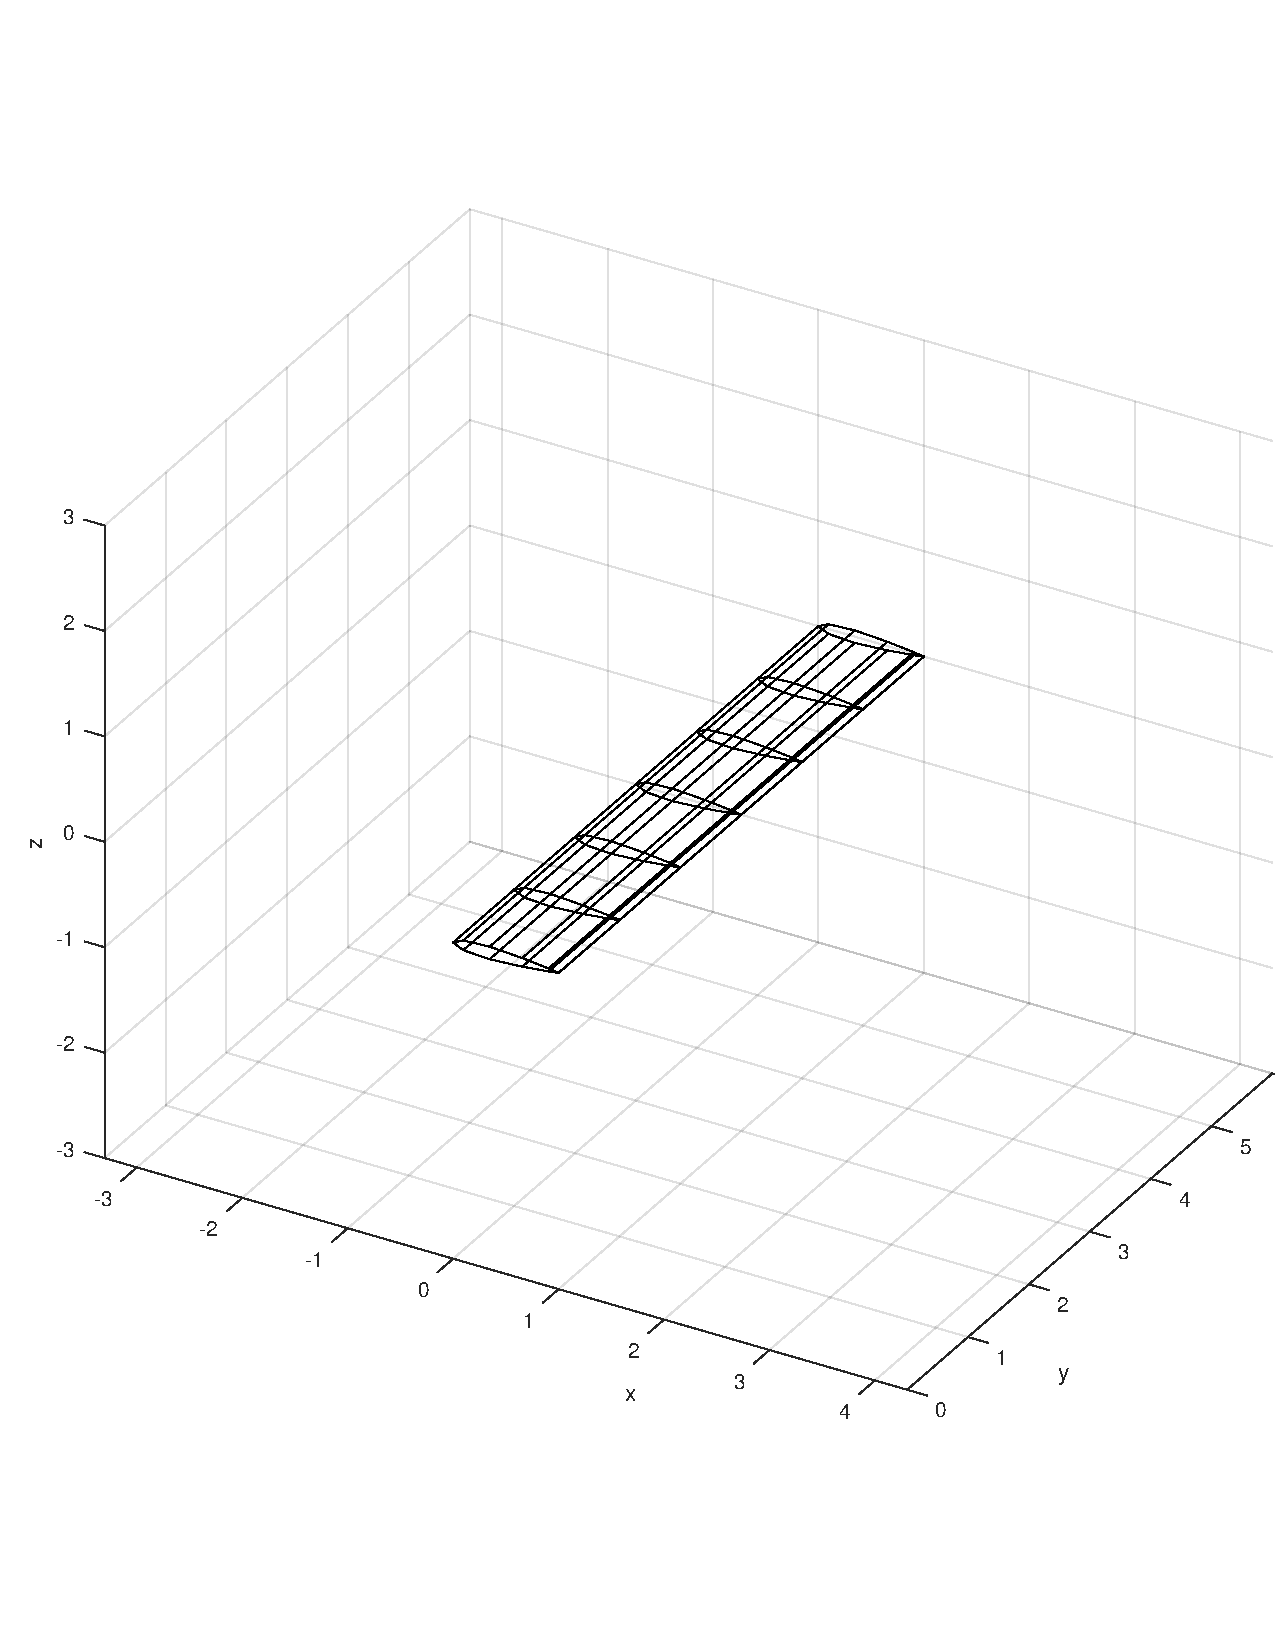
\includegraphics[width=.45\textwidth]{wing} \hspace{30pt}
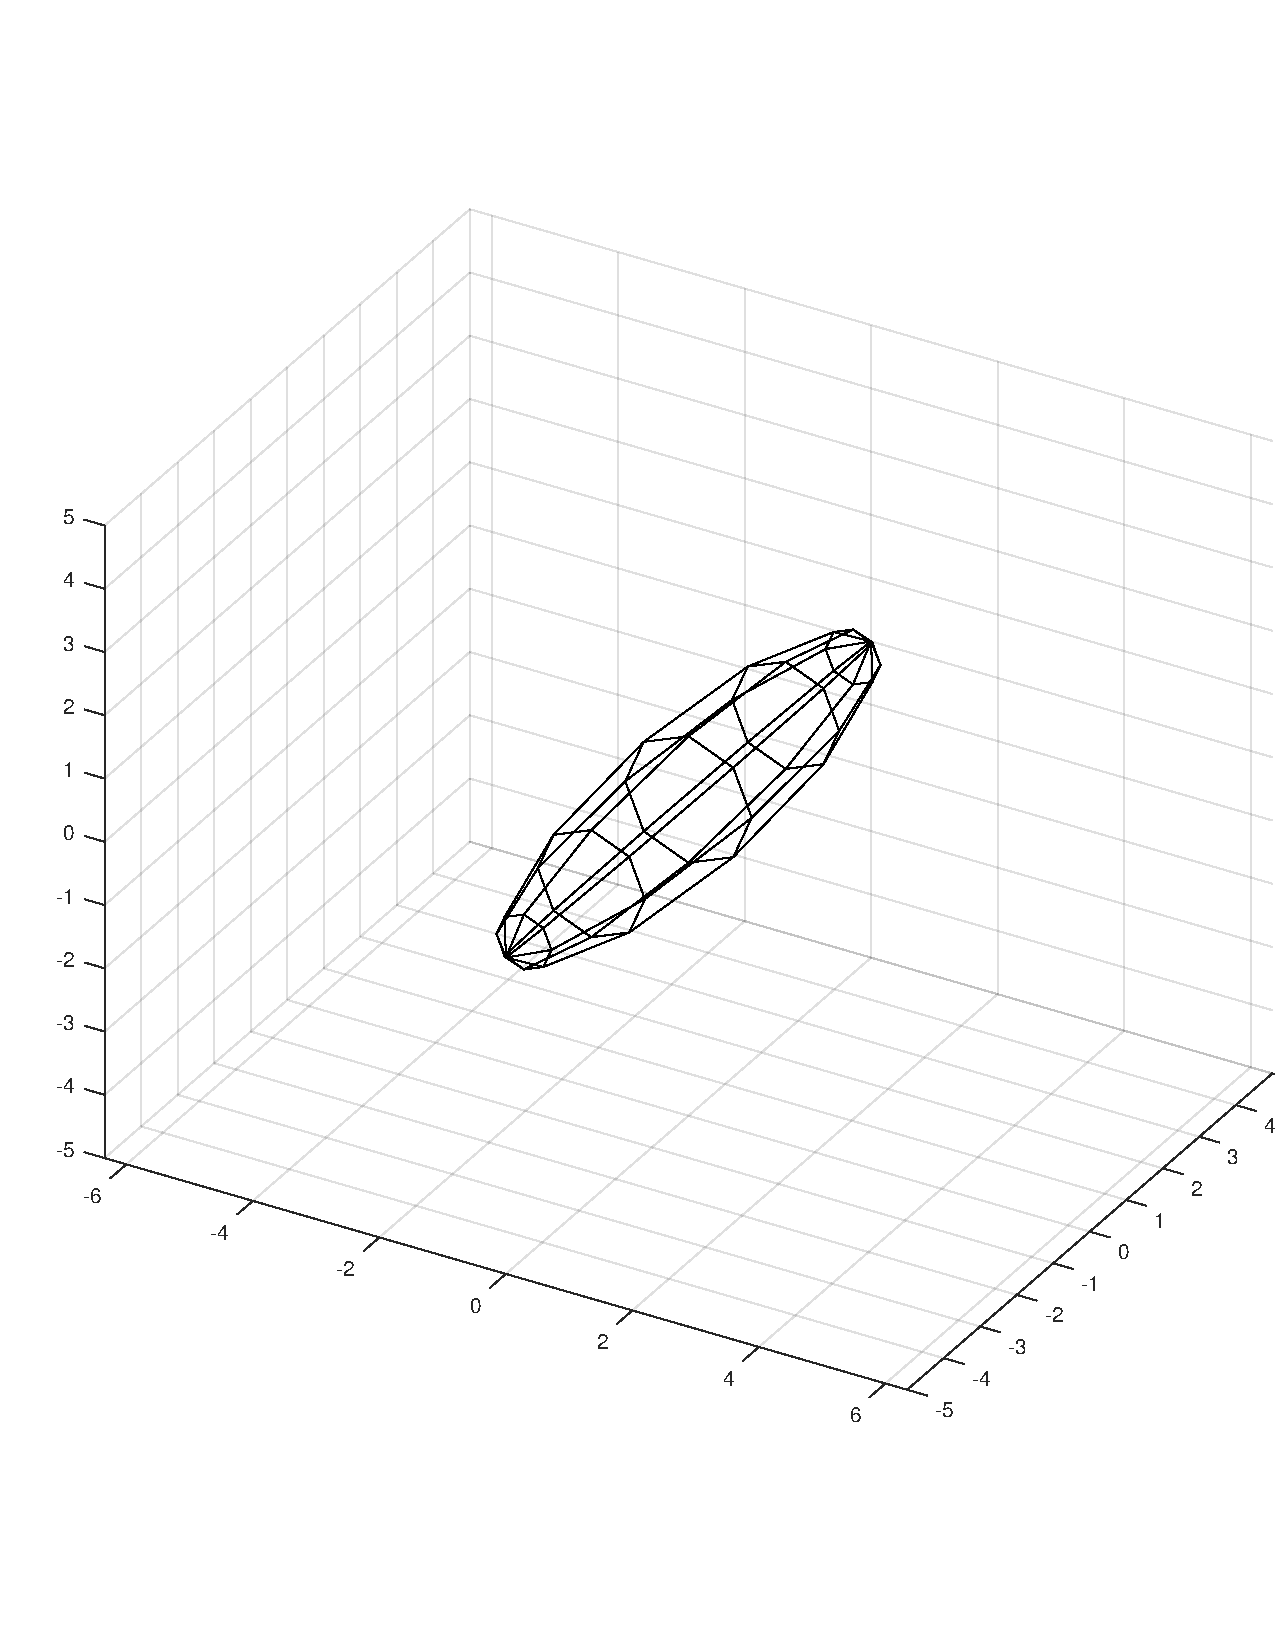
\includegraphics[width=.45\textwidth]{tank}
\caption{Components defined by means of basic mesh generations in the examples: wing and tank.}
\label{fig:basic_components_example}
\end{figure}
\newline
The following script \ref{file:wing_m} relies on the function \opt{setAirfoil4()} to define the two-dimensional airfoils and builds the basic input files for DUST of a rectangular wing with open tips.
\begin{inputfile}[frame=single, caption={\opt{wing.m}}, label={file:wing_m}]
% =========================================================================== %
% build the geometry and connectivity for a rectangular wing
% ( y-axis identifies the spanwise direction )
%
%  rr(3,n_points): array of the coordinates of the points of the surface
%  ee(4,n_elems ): array of the note-to-elem connectivity
% =========================================================================== %
clear all ; clc ; close all

% === params ===
chord      = 1.0 ;
span       = 6.0 ;
n_span_el  = 10  ;
n_chord_el = 5   ; % n_chord_el = n. elems on the chord

%> the tot. number of elems for a 3dpanel component ('p' in dust) is
n_elems = (n_span_el)*(2*n_chord_el) ;

%> the tot. number of points for a 3dpanel component ('p' in dust) is
n_points_per_sec = 2*n_chord_el+1 ;
n_points         = (n_span_el+1) * n_points_per_sec ;

%> vector of spanwise coord.s of the airfoil sections: uniform spacing, here
y_sec = linspace(0,span,(n_span_el+1)) ;

% === rr array ===
rr = zeros(n_points,3) ;

for i_sec = 1 : n_span_el+1

  %> define the 2d airfoil, NACA 4-digit airfoils, NACA-MPSS
  % setAirfoil ( M , P , SS , chord , n_chord_el , other parameters ... )
  [ x , z ] = setAirfoil4( 0 , 0 , 12 , chord , n_chord_el , ...
                           0.0 , 0.0 , 0.0 , 0.0 , 0 ) ; 
  %> update rr array
  rr(1+(i_sec-1)*n_points_per_sec:i_sec*n_points_per_sec,:) = ...
                                 [ x ; y_sec(i_sec)*ones(size(x)) ; z ]' ;
end

% === ee array ===
ee = zeros(n_elems,4) ; ie = 0 ;

for i_sec = 1 : n_span_el
  for i_p = 1 : n_points_per_sec-1

    ie = ie + 1 ;
    ee(ie,:) = [ i_sec   *n_points_per_sec+i_p   , ...
                 i_sec   *n_points_per_sec+i_p+1 , ...
                (i_sec-1)*n_points_per_sec+i_p+1 , ...
                (i_sec-1)*n_points_per_sec+i_p   ] ;
  end
end

% === check the connectivity with the Patch plot routine ===
% patch has rr,ee arrays as inputs --> easy way to check the rr,ee arrays
figure ; grid on ; axis equal
patch('Vertices',rr,'Faces',ee,'FaceColor','none')

% === save to .dat file in ascii format ===
%save('wing_rr.dat','rr','-ascii')
%save('wing_ee.dat','ee','-ascii')
dlmwrite('wing_rr.dat',rr, 'delimiter','\t')
dlmwrite('wing_ee.dat',ee, 'delimiter','\t')

\end{inputfile}
The files \ref{file:wing_rr} and \ref{file:wing_ee} are respectively the \opt{rr.dat} and \opt{ee.dat} files produced by the \opt{wing.m} script.

\begin{minipage}[]{0.48\textwidth}
 \begin{inputfile}[frame=single, caption={\opt{rr.dat} created by \opt{wing.m}}, label={file:wing_rr}]
    1.0000         0   -0.0013
    0.9045         0   -0.0139
    0.6545         0   -0.0409
    0.3455         0   -0.0596
    0.0955         0   -0.0460
         0         0         0
    0.0955         0    0.0460
    0.3455         0    0.0596
    0.6545         0    0.0409
    0.9045         0    0.0139
    1.0000         0    0.0013
    1.0000    1.0000   -0.0013
    0.9045    1.0000   -0.0139
    0.6545    1.0000   -0.0409
    0.3455    1.0000   -0.0596
    0.0955    1.0000   -0.0460
         0    1.0000         0
    0.0955    1.0000    0.0460
    0.3455    1.0000    0.0596
    0.6545    1.0000    0.0409
    0.9045    1.0000    0.0139
    1.0000    1.0000    0.0013
    1.0000    2.0000   -0.0013
    0.9045    2.0000   -0.0139
    0.6545    2.0000   -0.0409
    0.3455    2.0000   -0.0596
    0.0955    2.0000   -0.0460
         0    2.0000         0
    0.0955    2.0000    0.0460
    0.3455    2.0000    0.0596
    0.6545    2.0000    0.0409
    0.9045    2.0000    0.0139
    1.0000    2.0000    0.0013
    1.0000    3.0000   -0.0013
    0.9045    3.0000   -0.0139
   ...
    0.9045    6.0000    0.0139
    1.0000    6.0000    0.0013
 \end{inputfile}
\end{minipage} \hspace{10pt}
\begin{minipage}[]{0.48\textwidth}
 \begin{inputfile}[frame=single, caption={\opt{ee.dat} file created by \opt{wing.m}}, label={file:wing_ee}]
    12    13     2     1
    13    14     3     2
    14    15     4     3
    15    16     5     4
    16    17     6     5
    17    18     7     6
    18    19     8     7
    19    20     9     8
    20    21    10     9
    21    22    11    10
    23    24    13    12
    24    25    14    13
    25    26    15    14
    26    27    16    15
    27    28    17    16
    28    29    18    17
    29    30    19    18
    30    31    20    19
    31    32    21    20
    32    33    22    21
    34    35    24    23
    35    36    25    24
    36    37    26    25
    37    38    27    26
    38    39    28    27
    39    40    29    28
    40    41    30    29
    41    42    31    30
    42    43    32    31
   ...
    69    70    59    58
    70    71    60    59
    71    72    61    60
    72    73    62    61
    73    74    63    62
    74    75    64    63
    75    76    65    64
    76    77    66    65
 \end{inputfile}
\end{minipage}

 \noindent
The following script \ref{file:tank_m} builds the basic input files for DUST of a ellipsoidal tank with cylindrical sections.
\begin{inputfile}[frame=single, caption={\opt{tank.m}}, label={file:tank_m}]
% =========================================================================== %
% build the geometry and connectivity of a tank with ellipsoidal shape
% ( y-axis identifies the axial direction )
%
%  rr(3,n_points): array of the coordinates of the points of the surface
%  ee(4,n_elems ): array of the note-to-elem connectivity
%
%     /o----o--------o----o\
%    /_o----o--------o----o_\
%   o< -- . -- . -- . -- .  >o -- . -- axis
%    \ o----o--------o----o /
%     \o----o--------o----o/
%   sec.1   .2       .3   .4
% =========================================================================== %
clear all ; clc ; close all

% === params ===
a = 5.0 ; b = 1.0 ; % major and minor semi-axis of the cylindrical ellipsoid
n_axial_sec = 5   ; % n. cylindrical sections, excluding the tank extreme points
n_radial_el = 8   ; % n_chord_el = n. elems on the chord

%> the tot. number of elems for a 3dpanel component ('p' in dust) is
n_elems = n_radial_el * (n_axial_sec+1) ;

%> the tot. number of points for a 3dpanel component ('p' in dust) is
n_points_per_sec = n_radial_el ;
n_points = ...
  n_points_per_sec*n_axial_sec + 2 ; % + 2: for the extreme points

%> vector of spanwise coord. and radius of the tank sections
% here, ellipsoid with Chebychev spacing on the major axis
dth = pi/(n_axial_sec+2) ;
th_vec = linspace( pi-dth , dth , n_axial_sec ) ;
y_sec = a * cos(th_vec) ; 
r_sec = b * ( 1.0 - y_sec.^2 / a^2 ).^0.5 ;

%> extreme points y coord
y01 = - a ; y02 = a ;
 
% === rr array ===
rr = zeros(n_points,3) ; ir = 0 ;

for i_sec = 1 : n_axial_sec
  for i_p = 1 : n_points_per_sec

    %> update counter and find the th angle describing the polar coord
    ir = ir + 1 ;
    th = 2*pi*(i_p-1) / n_points_per_sec ;

    rr(ir,:) = [ r_sec(i_sec)*cos(th) , y_sec(i_sec) , r_sec(i_sec)*sin(th) ] ;

  end
end
%> update rr with the first and last point
rr = [ [ 0.0, -a, 0.0 ] ; rr(1:ir,:) ; [ 0.0, a, 0.0 ] ] ; 

% === ee array ===
ee = zeros(n_elems,4) ; ie = 0 ; % Initialisation to zero

%> first TRIA sector (last col remains equal to 0)
for i_p = 1 : n_points_per_sec

  ie = ie + 1 ;
  ee(ie,1:3) = [ 1 , 1+i_p , 1+mod(i_p,n_points_per_sec)+1 ] ;

end

%> inner QUAD sectors
for i_sec = 1 : n_axial_sec-1
  for i_p = 1 : n_points_per_sec

    ie = ie + 1 ;
    ee(ie,:) = int32([ 1+(i_sec-1)*n_points_per_sec+ i_p , ...
                 1+ i_sec   *n_points_per_sec+ i_p , ...
                 1+ i_sec   *n_points_per_sec+ mod(i_p,n_points_per_sec)+1 , ...
                 1+(i_sec-1)*n_points_per_sec+ mod(i_p,n_points_per_sec)+1 ]);
  end
end

%> first TRIA sector (last col remains equal to 0)
for i_p = 1 : n_points_per_sec

  ie = ie + 1 ;
  ee(ie,1:3) = int32([1+(n_axial_sec-1)*n_points_per_sec+i_p , ...
                n_points , ...
                1+(n_axial_sec-1)*n_points_per_sec+mod(i_p,n_points_per_sec)+1]);
                 
end

% === save to .dat file in ascii format (OCTAVE) ===
save('tank_rr.dat','rr','-ascii')
save('tank_ee.dat','ee','-ascii')
% === save to .dat file in ascii format (MATLAB) ===
dlmwrite('tank_rr.dat',rr, 'delimiter','\t')
dlmwrite('tank_ee.dat',ee, 'delimiter','\t')


% === check the connectivity with the Patch plot routine ===
% patch has rr,ee arrays as inputs --> easy way to check the rr,ee arrays
%> patch does not allow 0 indices in ee -> substitute 4th zero el with 3rd el
for ie = 1 : n_elems
 if ( ee(ie,4) == 0 ) ; ee(ie,4) = ee(ie,3) ; end 
end

figure ; grid on ; axis equal
patch('Vertices',rr,'Faces',ee,'FaceColor','none')

\end{inputfile}

\noindent
The files \ref{file:tank_rr} and \ref{file:tank_ee} are respectively the \opt{rr.dat} and \opt{ee.dat} files of the ellipsoidal tank, generated by the \opt{tank.m} script \ref{file:tank_m}.

\begin{minipage}[t]{0.48\textwidth}
 \begin{inputfile}[frame=single, caption={\opt{rr.dat} file created by \opt{tank.m}}, label={file:tank_rr}]
         0   -5.0000         0
    0.4339   -4.5048         0
    0.3068   -4.5048    0.3068
    0.0000   -4.5048    0.4339
   -0.3068   -4.5048    0.3068
   -0.4339   -4.5048    0.0000
   -0.3068   -4.5048   -0.3068
   -0.0000   -4.5048   -0.4339
    0.3068   -4.5048   -0.3068
    0.8467   -2.6602         0
    0.5987   -2.6602    0.5987
    0.0000   -2.6602    0.8467
   -0.5987   -2.6602    0.5987
   -0.8467   -2.6602    0.0000
   -0.5987   -2.6602   -0.5987
   -0.0000   -2.6602   -0.8467
    0.5987   -2.6602   -0.5987
    1.0000    0.0000         0
    0.7071    0.0000    0.7071
    0.0000    0.0000    1.0000
   -0.7071    0.0000    0.7071
   -1.0000    0.0000    0.0000
   -0.7071    0.0000   -0.7071
   -0.0000    0.0000   -1.0000
    0.7071    0.0000   -0.7071
    0.8467    2.6602         0
    0.5987    2.6602    0.5987
    0.0000    2.6602    0.8467
   -0.5987    2.6602    0.5987
   -0.8467    2.6602    0.0000
   -0.5987    2.6602   -0.5987
   -0.0000    2.6602   -0.8467
    0.5987    2.6602   -0.5987
    0.4339    4.5048         0
    0.3068    4.5048    0.3068
    0.0000    4.5048    0.4339
   -0.3068    4.5048    0.3068
   -0.4339    4.5048    0.0000
   -0.3068    4.5048   -0.3068
   -0.0000    4.5048   -0.4339
    0.3068    4.5048   -0.3068
         0    5.0000         0
 \end{inputfile}
\end{minipage} \hspace{10pt}
\begin{minipage}[t]{0.48\textwidth}
 \begin{inputfile}[frame=single, caption={\opt{ee.dat} file created by \opt{tank.m}}, label={file:tank_ee}]
     1     2     3     0
     1     3     4     0
     1     4     5     0
     1     5     6     0
     1     6     7     0
     1     7     8     0
     1     8     9     0
     1     9     2     0
     2    10    11     3
     3    11    12     4
     4    12    13     5
     5    13    14     6
     6    14    15     7
     7    15    16     8
     8    16    17     9
     9    17    10     2
    10    18    19    11
    11    19    20    12
    12    20    21    13
    13    21    22    14
    14    22    23    15
    15    23    24    16
    16    24    25    17
    17    25    18    10
    18    26    27    19
    19    27    28    20
    20    28    29    21
    21    29    30    22
    22    30    31    23
    23    31    32    24
    24    32    33    25
    25    33    26    18
    26    34    35    27
    27    35    36    28
    28    36    37    29
    29    37    38    30
    30    38    39    31
    31    39    40    32
    32    40    41    33
    33    41    34    26
    34    42    35     0
    35    42    36     0
    36    42    37     0
    37    42    38     0
    38    42    39     0
    39    42    40     0
    40    42    41     0
    41    42    34     0
 \end{inputfile}
\end{minipage} \hspace{10pt}



\section{Parametric mesh generation}
\label{sec:Parametric_mesh_generation}

The parametric mesh generation has the aim of allowing the generation of slender bodies, mainly wings, to be generated parametrically in the preprocessor with few directives, without resorting to an external mesh generator. 

To generate the parametric geometry a geometry input file to be referenced in the preprocessor input file \ref{file:dust_pre.in} is employed. The input file is similar to the geometry files for standard meshes described in file \ref{file:geo_file.in}


\subsection{Surface panels and vortex lattices}

\begin{inputfile}[frame=single, caption={paramtetric\_geo\_file.in}, label={file:parametric_geo_file.in}]
mesh_file_type = parametric
el_type = v

scaling_factor = 1.0
offset = (/0.0, 0.0, 0.0/)

AirfoilTableCorrection = T

mesh_symmetry = F
symmetry_point  = (/0.0, 0.0, 0.0/)
symmetry_normal = (/0.0, 1.0, 0.0/)

mesh_mirror = F
mirror_point  = (/0.0, 0.0, 0.0/)
mirror_normal = (/1.0, 0.0, 0.0/)

twist_linear_interpolation = F

starting_point = (/0.0,0.0865,0.0/)
reference_chord_fraction = 0.0

!mesh_flat = T

nelem_chord = 10
type_chord = cosineLE

! First section
chord = 1.0
twist = -1.0
airfoil_table = ./airfoils/naca0012.c81
airfoil = NACA0012

! First region
span = 0.5
sweep = 0.0
dihed = 0.0
nelem_span = 3 
type_span = uniform

! Second section
chord = 1.0
twist = 0.0
airfoil = interp

! Second region
span = 4.0
sweep = 10.0
dihed = 5.0
nelem_span = 10 
type_span = uniform

! Third section
chord = 0.5
twist =  0.0
airfoil_table = ./airfoils/naca0012.c81
airfoil = NACA0012

\end{inputfile}

The parametric geometry is obtained by connecting with a surface different planar sections. With the planar sections the user defines the shape of the section, the chord and the twist of the section. Then sections are connected by regions, with which the number of span panels, span, dihedral and sweep are defined. The user can define an arbitrary number $n_s$ of sections, which must then be connected with $n_s-1$ regions. A representation of sections and regions employed for the generation of a wing is presented in figure \ref{fig:parametric_wing}. The body is generated from the first section, starting from the specified starting point, and it is extruded along the y axis, with the x axis pointing from the leading edge towards the trailing edge and the z axis normal to the x-y plane. 
The type of geometry generated depends on the type of elements required. If surface panels are required the full three dimensional geometry will be generated, if vortex lattice elements are required only the flat, mean line surface will be generated and finally if lifting line elements are required only a one dimensional line will be generated. Finally the mirroring of the geometry introduced for user generated meshes is available also for parametric geometries.

All the detailed parameters of the geometry input file for parametric geometry are:
\begin{itemize}
\item \param{mesh_file_type}: \textit{required:} yes. \textit{multiple:} no. \textit{type:} string. 

Use \param{parametric} for parametric geometry.

\item \param{el_type}: \textit{required:} yes. \textit{multiple:} no. \textit{type:} character.

type of the elements of the mesh. \opt{p} stands for surface panels to model solid bodies, \opt{v} stands for vortex lattice elements used to model flat surfaces, \opt{l} stands for lifting lines used to produce a 1D model of a lifting surface. 

\item \param{offset} \textit{required:} no. \textit{multiple:} no. \textit{default:} (0.0, 0.0, 0.0) \textit{type:} real array, length 3.

offset to apply to the loaded points. Allows to move the coordinates of the loaded points of the vector specified. 

\item \param{scaling_factor} \textit{required:} no. \textit{multiple:} no. \textit{default:} 1.0 \textit{type:} real.

Scaling factor to apply to the loaded points. Allows to scale the coordinates of the loaded points of the specified factor.

offset and scaling are applied in the following order:
\begin{equation*}
\mathbf{r} = Scaling (\mathbf{r}_{loaded}+offset)
\end{equation*}


\item \param{AirfoilTableCorrection}: \textit{required:} yes. \textit{multiple:} no. \textit{type:} logical.

Require the viscous correction for \opt{v} elements by introducing the c81 aerodynamic tables. (Still experimental) 


\item \param{mesh\_symmetry} \textit{required:} no. \textit{multiple:} no. \textit{default:} false. \textit{type:} logical.

Choose to reflect the mesh around a point and a direction. Useful to produce full meshes out of symmetrical half models. Keeps both the original and the symmetrical part. 

\item \param{symmetry\_point}: \textit{required:} only if \param{mesh\_reflection} is true. \textit{multiple:} no. \textit{default:} (0.0, 0.0, 0.0). \textit{type:} real array, length 3.

point around which to reflect the mesh.

\item \param{symmetry\_normal}: \textit{required:} only if \param{mesh\_reflection} is true. \textit{multiple:} no. \textit{default:} (0.0, 1.0, 0.0). \textit{type:} real array, length 3.

Direction in which to reflect the mesh.

\item \param{mesh\_mirror} \textit{required:} no. \textit{multiple:} no. \textit{default:} false. \textit{type:} logical.

Choose to mirror the mesh around a point and a direction. Same as \param{mesh\_symmetry} but does not keep both the original, i.e. the mesh is not doubled.

\item \param{mirror\_point}:  \textit{required:} only if \param{mesh\_reflection} is true. \textit{multiple:} no. \textit{default:} (0.0, 0.0, 0.0). \textit{type:} real array, length 3.

point around which to mirror the mesh.

\item \param{mirror\_normal}: \textit{required:} only if \param{mesh\_reflection} is true. \textit{multiple:} no. \textit{default:} (0.0, 1.0, 0.0). \textit{type:} real array, length 3.

Direction in which to mirror the mesh.

\item \param{twist\_linear\_interpolation} \textit{required:} no. \textit{multiple:} no. \textit{default:} false. \textit{type:} logical.

Choose to apply linear interpolation to the twist angle, instead of interpolating the point coordinates between two neighboring sections defined in the input file.

\item \param{starting\_point} \textit{required:} no. \textit{multiple:} no. \textit{default:} (/ 0.0, 0.0, 0.0 /) \textit{type:} real array, length 3.

point in the local reference frame in which to start extruding the parametric geometry.

\item \param{reference\_chod\_fraction} \textit{required:} no. \textit{multiple:} no. \textit{default:} 0.0 \textit{type:} real

Fraction of the chord at which to place the axis which will be rotated of the sweep and dihedral angles, and around which airfoils are twisted. 

\item \param{mesh\_flat} \textit{required:} no. \textit{multiple:} no. \textit{default:} true \textit{type:} logical

Used only in case of lifting lines (\opt{l}) elements. If enabled instead of generating lifting lies actually twisted according to the input twist, but rather a flat surface with only the normal vectors twisted according to the input twist. 

\item \param{nelem\_chord} \textit{required:} yes, if parametric. \textit{multiple:} no. \textit{type:} integer.

Number of elements in chord direction. Note: if the elements are vortex lattice $nelem\_chord$ elements will be generated, while in case of surface panels $2nelem\_chord$ elements will be produced, $nelem\_chord$ on the lower and $nelem\_chord$ on the upper side. In case of lifting lines this parameter is ignored.

\item \param{type\_chord} \textit{required:} no. \textit{multiple:} no. \textit{default:} uniform \textit{type:} string.

type of subdivision in the chord-wise direction. Can be \opt{uniform} for a uniform distribution, \opt{cosine} for a cosine distribution, refined both on the leading and trailing edge, \opt{cosineLE} for a half cosine refined only on leading edge or \opt{cosineTE} for a half cosine refined only on the trailing edge. 

\item \param{chord} \textit{required:} at least 2. \textit{multiple:} yes. \textit{type:} real.

Defines a section, by its chord length

\item \param{twist} \textit{required} in same number as \param{chord}. \textit{multiple} yes. \textit{type:} real.

Angle of twist, in degrees, of the airfoil section.

\item \param{airfoil}/\param{airfoil\_table} \textit{required:} in same number as \param{chord}. \textit{multiple:} yes. \textit{type:} string.

airfoil of the section. There are different ways to define an airfoil. It can be defined by the user as a series of points, and so \param{airfoil} must be the path to a .dat file (the extension is mandatory) containing the two dimensional coordinates of an airfoil; the file must have in the first line an integer representing the number of points provided, followed by the coordinates of each point on separate lines. It can also be an analytical NACA profile, and so must be provided as a NACAXXXX string (at the moment only 4 digits and some 5 digits are implemented). 

In case of lifting lines or when \param{AirfoilTableCorrection} is true on the vortex lattice, to mark the difference the \param{airfoil\_table} must be employed, and it refers to the path to the corresponding c81 lookup table. 

Optionally in the \param{airfoil} or \param{airfoil\_table} parameter it is possible to specify the option \opt{interp}. In this case the airfoil (airfoil section, mean line, section defined from file or c81 lookup table according to the type of elements) in the section will be linearly interpolated among the pair of explicitly specified airfoils in which the section is contained. 

\item \param{span} \textit{required:} at least one, in same number as \param{chord}-1 \textit{multiple:} yes. \textit{type:} real.

Define the span length of the region between two sections.  

\item \param{sweep} \textit{required:} in same number as \param{span} \textit{multiple:} yes. \textit{type:} real.

Angle of sweep of the region, positive if swept backwards (towards positive x).

\item \param{dihed} \textit{required:} in same number as \param{span} \textit{multiple:} yes. \textit{type:} real.

Angle of dihedral of the region, positive if rotated upwards (towards positive z).

\item \param{nelem\_span} \textit{required:} in same number as \param{span} \textit{multiple:} yes. \textit{type:} integer.

Number of elements in the spanwise direction, in the single region.

\item \param{type\_span} \textit{required:} in same number as \param{span} \textit{multiple:} yes. \textit{type:} string.

type of refinement of the elements in the spanwise direction. As for the chordwise direction, the options are \opt{uniform} for a uniform distribution, \opt{cosine} for a cosine refinement both inboard and outboard, and \opt{cosineIB} and \opt{cosineOB} for half cosine refinement only inboard or outboard. 
  
\end{itemize}

%TODO: actuator disk?

The concept of sections and regions is illustrated in figure \ref{fig:parametric_wing}. Furthermore an example to understand the geometrical role of the parameters in the input file is presented in file \ref{file:parametric_example_file.in} and figure \ref{fig:parametric_sections}.

\begin{figure}[h]
\centering
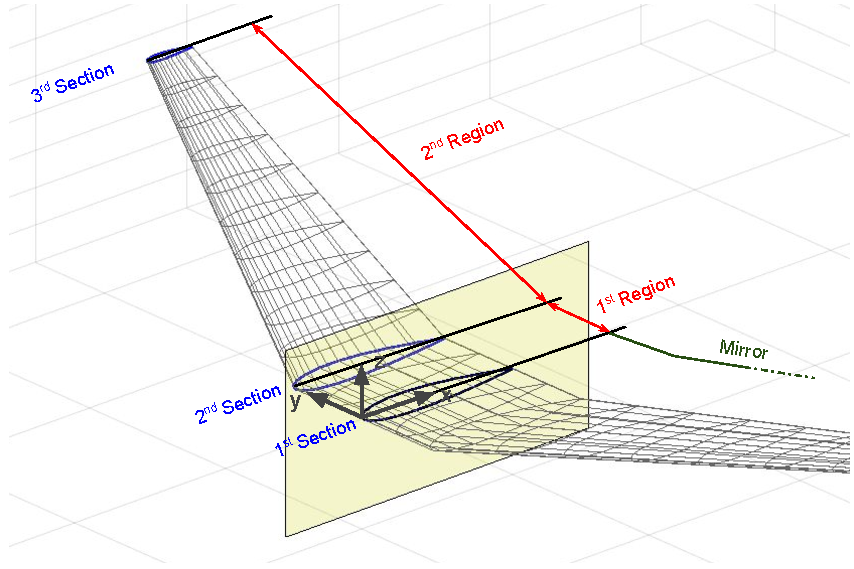
\includegraphics[width=.7\textwidth]{parametric_wing}
\caption{Sections and regions in parametric wing generation}
\label{fig:parametric_wing}
\end{figure}

When generating the parametric geometry, the slender body is generated starting from the \param{starting\_point} and then develops in the y direction (in the local reference frame of the component), with deviations induced by the various angles used as input. 

From the \param{starting\_point} a segmented reference line is created, in blue in figure \ref{fig:parametric_sections}. Each segment, which creates a region as in figure \ref{fig:parametric_wing}, is created from the previous node, is long \param{span} and is angled from the local component y direction of \param{dihed} dihedral angle with respect to the horizontal plane (rotating around the local x axis, positive upward, red in the figure) and of \param{sweep} angle with respect to the vertical plane (rotating around the local z axis, positive backward towards x, green in figure). 

Then on each node the airfoil section is applied, 2 dimensional for surface panels (as in figure) mono dimensional for vortex lattices (lifting lines will be discussed afterwards). The section is collocated so that the reference line passes through a certain \param{reference\_chord\_fraction} of the airfoil chord. Then the section is rotated around such point of a \param{twist} angle (around the component local y axis, positive when creating a positive pitch to the airfoils, in magenta in the figure). 

Finally all the sections are connected with the appropriate number of elements, as shown in figure \ref{fig:parametric_wing}.

\begin{figure}[h]
\centering
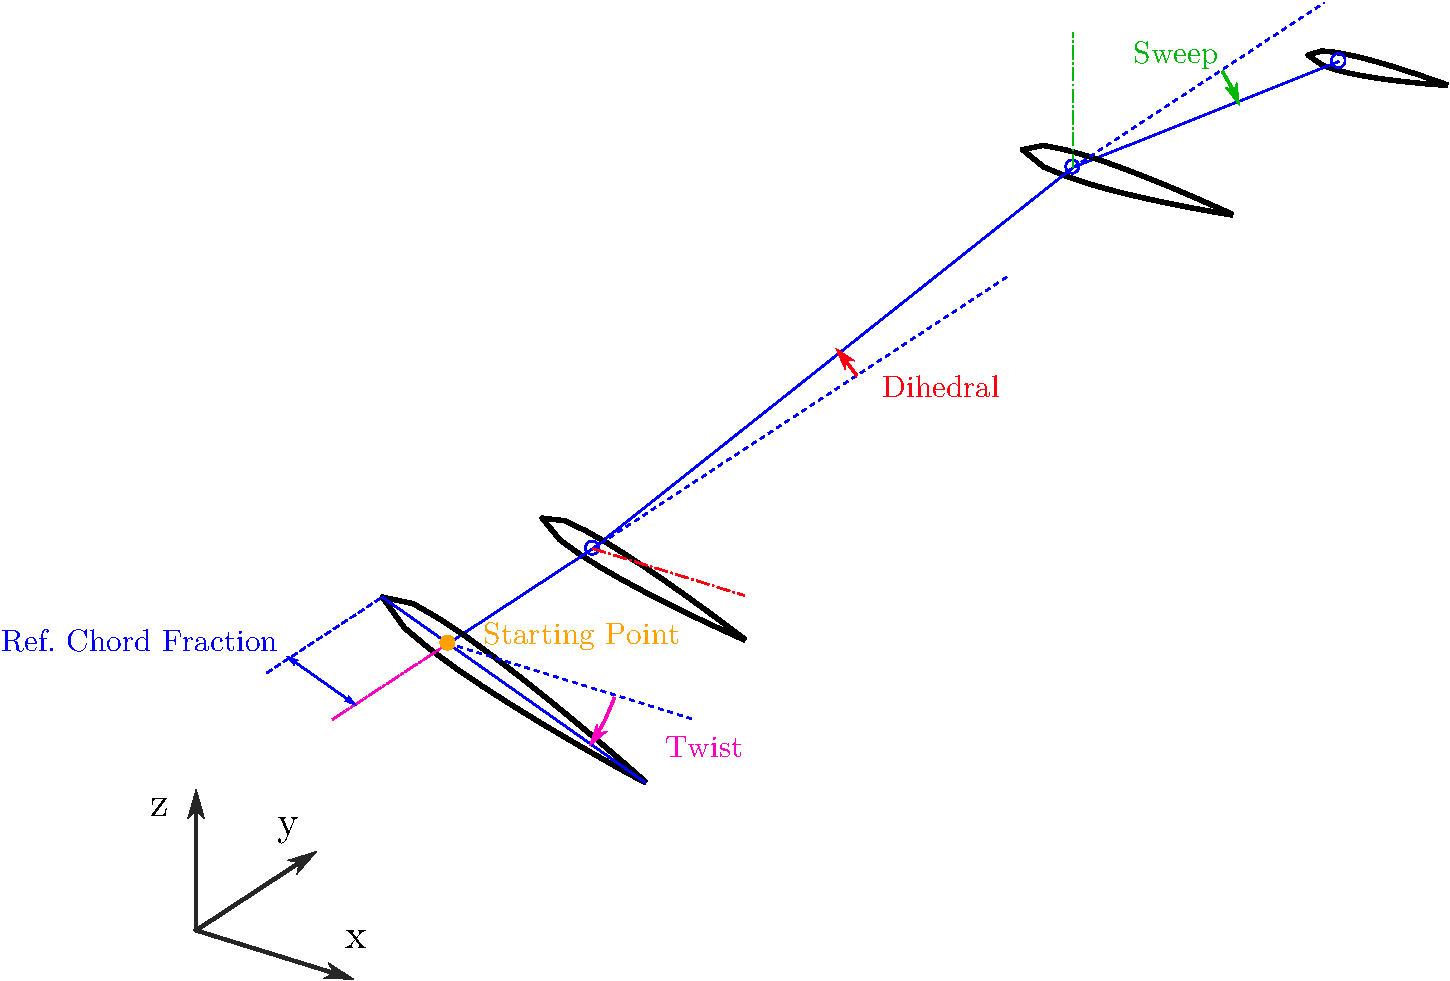
\includegraphics[width=.7\textwidth]{parametric_sections}
\caption{Generation logic of the geometry of parametric elements, generated from input file \ref{file:parametric_example_file.in}}
\label{fig:parametric_sections}
\end{figure}

\begin{inputfile}[frame=single, caption={Parametric geometry for figure \ref{fig:parametric_sections}}, label={file:parametric_example_file.in}]
mesh_file_type = parametric
el_type = p

nelem_chord = 10
type_chord = uniform   ! uniform  cosineLE  cosineTE

scaling_factor = 1.0
offset = (/0.0, 0.0, 0.0/)

starting_point = (/0.0,0.0,0.0/)
reference_chord_fraction = 0.25

! section 1
chord = 2.0
twist = 20.00
airfoil = NACA0012

! region  1
span = 1.5
sweep = 0.0
dihed = 0.0
nelem_span = 15
type_span = uniform

! section 2
chord = 1.5
twist = 15.0
airfoil = NACA0012

! region  2
span = 5.0
sweep = 0.0
dihed = 5.0
nelem_span = 50
type_span = uniform

! section 3
chord = 1.5
twist = 0.0
airfoil = NACA0012

! region  3
span = 2.0
sweep = 15.0
dihed = 0.0
nelem_span = 20
type_span = uniform

! section 4
chord = 1.0
twist = -5
airfoil = NACA0012
\end{inputfile}


\subsection{Airfoils sections geometry}
The airfoils sections, introduced with the keyword \param{airfoil}, as previously discussed, can be introduced either by specifying a NACA airfoil shape, or by providing a two dimensional geometry using an ascii file. In both cases the resulting number of points in the section is the one defined in \param{nelem\_chord}, with the distribution specified in \param{type\_chord}. 

In case of NACA airfoils, only 4 digits NACA airfoils and some 5 digits ones are implemented. When surface panels are employed the full shape is discretized, while when employing vortex lattices only the camber line is used to discretize the surface. 

In case of user provided geometry, the geometry must be provided as an ascii file with the coordinates used to describe the shape to be discretized. To mark the use of the user-defined shape the file name must have the extension \texttt{.dat}. 
The first line of the file must contain a single integer, which represents the number of points used to describe the shape, and thus the number of following lines. 
The next lines must contain two real numbers on each line, representing the x and y coordinates of each point. The horizontal, streamwise x axis points  towards the trailing edge, and the vertical y axis points upwards. 

The order in which the points are provided defines the direction of the curve that defines the shape of the airfoil. For vortex lattices the curve must start at the leading edge and end at the trailing edge, from which the wake will detach. For three dimensional surface panel the curve must start at the trailing edge, pass from the lower side of the airfoil, the leading edge, the upper side and end again at the trailing edge. The first and last point can be not coinciding, to generate an open trailing edge. 

In both vortex lattices and surface panels the input is assumed to be normalized to have an unit chord, the final chord of the geometry will be generated by multiplying by the \param{chord} parameter the coordinates (thus if the geometry provided is not normalized to have a unit chord, the actual chord obtained will be different from the value specified in \param{chord}).

An example of user prescribed airfoil shape is provided in file \ref{file:airfoil_shape.dat}.

\begin{inputfile}[frame=single, caption={Example of user specified airfoil shape (the middle lines have been suppressed for brevity)}, label={file:airfoil_shape.dat}]
72
1.0      0.0   
0.996103      -1.3540067E-4   
0.984179      -3.5814368E-4   
0.964464      -1.693276E-4   
0.937582      -5.391884E-4   
0.904605      -0.0017722012   
0.866738      -0.0038649566   
...
...
...
0.948453      0.013156898   
0.96962      0.0077201095   
0.985778      0.00345874   
0.996349      8.9363643E-4   
1.0      0.0   
\end{inputfile}

\subsection{Lifting lines}

The geometrical logic for the generation of lifting lines is similar to the one for surface panels or vortex lattices, and differs in only few details. An example of the same geometry defined in file \ref{file:parametric_example_file.in} and depicted in figure \ref{fig:parametric_sections} but generated as lifting lines is presented in figure \ref{fig:parametric_sections_ll}. When employing lifting lines the reference line is generated starting from the \param{starting\_point} exactly in the same way as in the other cases, however in this case this line is the one that will become the lifting line. From the lifting line a single panel is generated to represent the object surface, and implicitly the first wake panel. The panel is long 75\% of the indicated chord, and it is angled according to the \param{twist} angle set in the input. Therefore note that in case of lifting lines the lifting line is essentially always placed at 25\% of the ideal airfoil it should represent, and that the parameter \param{reference\_chord\_fraction} is ignored. 

\begin{figure}[h]
\centering
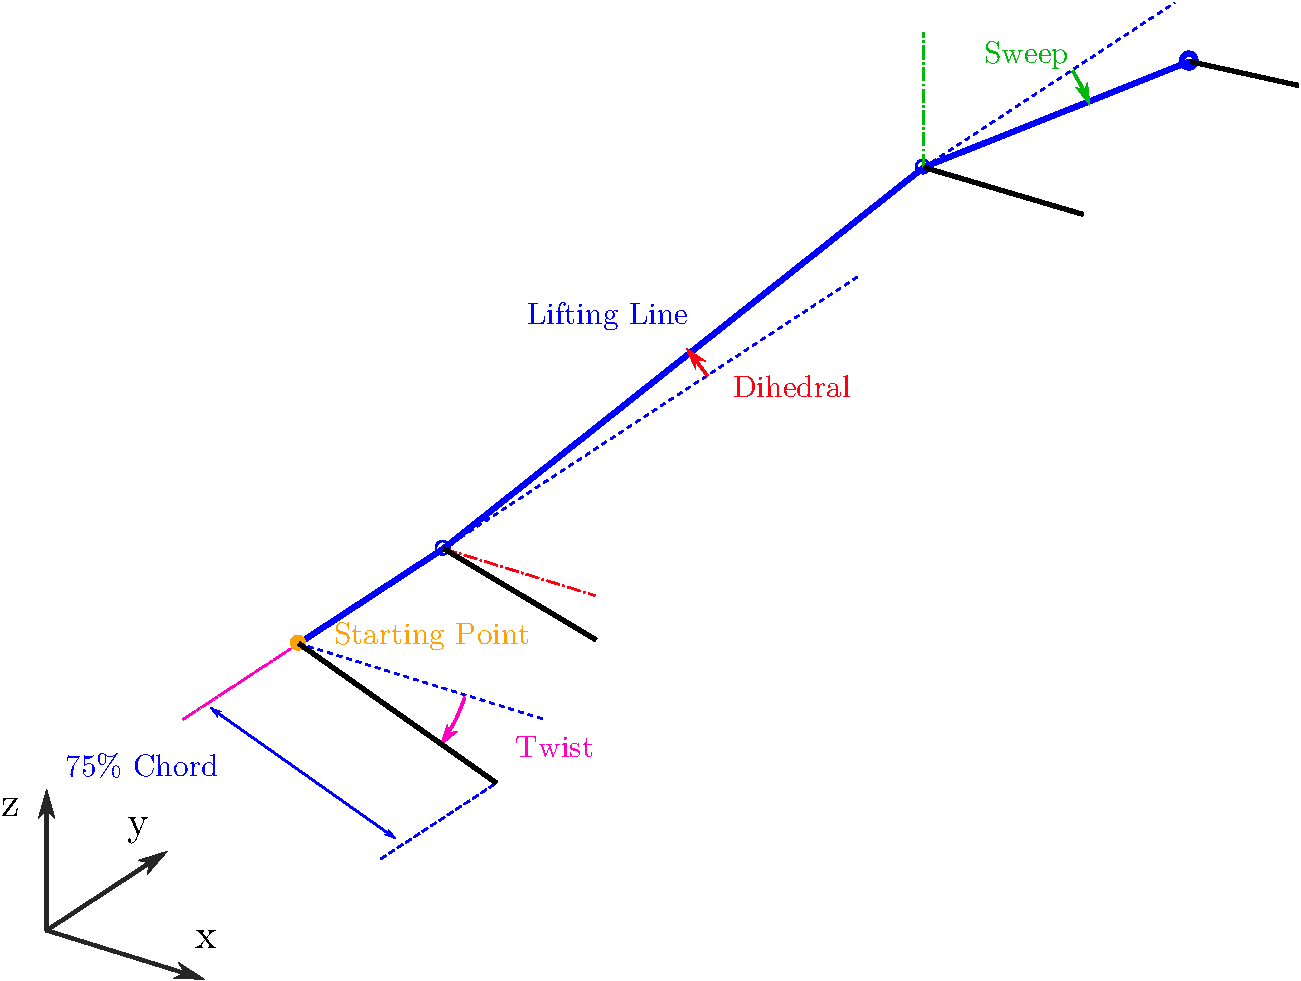
\includegraphics[width=.7\textwidth]{parametric_sections_ll}
\caption{Generation logic of the geometry of parametric lifting lines.}
\label{fig:parametric_sections_ll}
\end{figure}

Finally it is important to stress that the reference frames introduced in the present section concerning the generation of parametric components are local to those component, and are required only to assign coordinates to the points generated parametrically, just as a mesh generated from CAD files and an external mesher will generate points in a certain reference frame. The actual position of the component in space during the simulation depends on the reference frame in which the component will be introduced. Reference frames employed during the simulation are discussed in section \ref{sec:Solver_ReferenceFrames}.

\subsection{Hinged Surfaces}
\label{sec:Hinge_surfaces}
It is possible to introduce one or more movable surfaces in the parametric definition of a wing.
As outlined by the scheme in Fig. \ref{fig:hinge} left, in a two-dimensional problem the control surface can be defined in the local reference frame of the component, by means of the hinge axis position $H$, the chordwise direction $\xi$ and a blending region $[-u, u]$ (defined by \param{hinge\_Offset} parameter)introduced to avoid irregular behavior of the mesh along with the rotation angle $\theta$.
\begin{figure}[htbp]
\vspace{-3cm}
\centering
    \def\svgwidth{\columnwidth}
    %% Creator: Inkscape inkscape 0.92.4, www.inkscape.org
%% PDF/EPS/PS + LaTeX output extension by Johan Engelen, 2010
%% Accompanies image file 'hinges.eps' (pdf, eps, ps)
%%
%% To include the image in your LaTeX document, write
%%   \input{<file_name>.pdf_tex}
%%  instead of
%%   \includegraphics{<file_name>.pdf}
%% To scale the image, write
%%   \def\svgwidth{<desired width>}
%%   \input{<file_name>.pdf_tex}
%%  instead of
%%   \includegraphics[width=<desired width>]{<file_name>.pdf}
%%
%% Images with a different path to the parent latex file can
%% be accessed with the `import' package (which may need to be
%% installed) using
%%   \usepackage{import}
%% in the preamble, and then including the image with
%%   \import{<path to file>}{<file_name>.pdf_tex}
%% Alternatively, one can specify
%%   \graphicspath{{<path to file>/}}
%% 
%% For more information, please see info/svg-inkscape on CTAN:
%%   http://tug.ctan.org/tex-archive/info/svg-inkscape
%%
\begingroup%
  \makeatletter%
  \providecommand\color[2][]{%
    \errmessage{(Inkscape) Color is used for the text in Inkscape, but the package 'color.sty' is not loaded}%
    \renewcommand\color[2][]{}%
  }%
  \providecommand\transparent[1]{%
    \errmessage{(Inkscape) Transparency is used (non-zero) for the text in Inkscape, but the package 'transparent.sty' is not loaded}%
    \renewcommand\transparent[1]{}%
  }%
  \providecommand\rotatebox[2]{#2}%
  \newcommand*\fsize{\dimexpr\f@size pt\relax}%
  \newcommand*\lineheight[1]{\fontsize{\fsize}{#1\fsize}\selectfont}%
  \ifx\svgwidth\undefined%
    \setlength{\unitlength}{489.93968126bp}%
    \ifx\svgscale\undefined%
      \relax%
    \else%
      \setlength{\unitlength}{\unitlength * \real{\svgscale}}%
    \fi%
  \else%
    \setlength{\unitlength}{\svgwidth}%
  \fi%
  \global\let\svgwidth\undefined%
  \global\let\svgscale\undefined%
  \makeatother%
  \begin{picture}(1,0.43599908)%
    \lineheight{1}%
    \setlength\tabcolsep{0pt}%
    \put(0,0){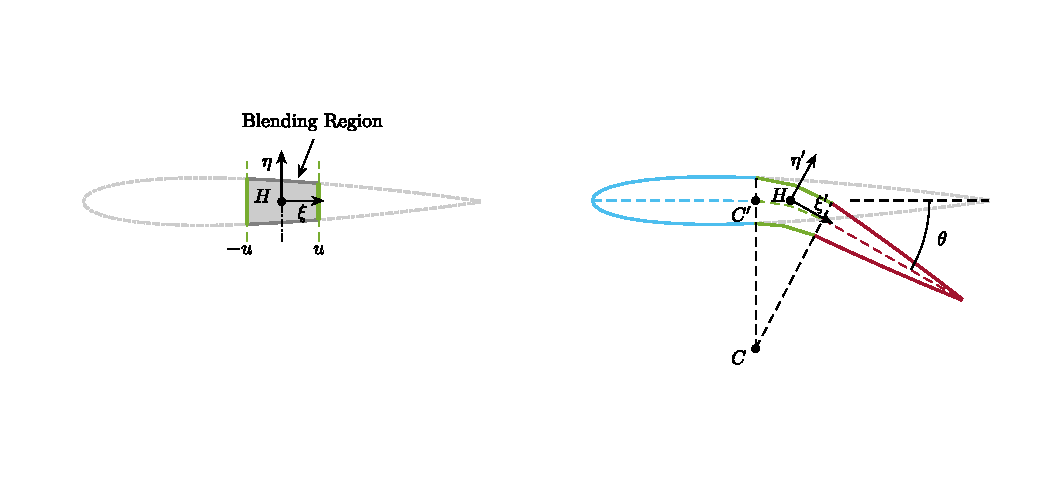
\includegraphics[trim={0 1.5cm 0 1.5cm},clip, width=\unitlength]{./images/hinges.eps}}%
  \end{picture}%
\endgroup%

    \caption{Scheme of the two-dimensional hinged surface configuration}
    \label{fig:hinge}
\end{figure}
Three regions are defined using the coordinates defined through this reference frame:
\begin{enumerate}
 \item $\xi \leq -u$: no influence of the aileron rotation;
 \item $\xi \geq  u$: rigid rotation around the hinge;
 \item $-u \le \xi \le  u$: blending region for avoiding irregular behavior defined as an arc of a circle whose center is locate on point $C$;
\end{enumerate}
In a three-dimensional problem, the reference configuration of a control surface, as an aileron, is defined in wind axis reference frame of the component.
\begin{figure}[htbp]
    \centering
    \def\svgwidth{\columnwidth}
    %% Creator: Inkscape inkscape 0.92.4, www.inkscape.org
%% PDF/EPS/PS + LaTeX output extension by Johan Engelen, 2010
%% Accompanies image file 'hinge_ref_system.pdf' (pdf, eps, ps)
%%
%% To include the image in your LaTeX document, write
%%   \input{<filename>.pdf_tex}
%%  instead of
%%   \includegraphics{<filename>.pdf}
%% To scale the image, write
%%   \def\svgwidth{<desired width>}
%%   \input{<filename>.pdf_tex}
%%  instead of
%%   \includegraphics[width=<desired width>]{<filename>.pdf}
%%
%% Images with a different path to the parent latex file can
%% be accessed with the `import' package (which may need to be
%% installed) using
%%   \usepackage{import}
%% in the preamble, and then including the image with
%%   \import{<path to file>}{<filename>.pdf_tex}
%% Alternatively, one can specify
%%   \graphicspath{{<path to file>/}}
%% 
%% For more information, please see info/svg-inkscape on CTAN:
%%   http://tug.ctan.org/tex-archive/info/svg-inkscape
%%
\begingroup%
  \makeatletter%
  \providecommand\color[2][]{%
    \errmessage{(Inkscape) Color is used for the text in Inkscape, but the package 'color.sty' is not loaded}%
    \renewcommand\color[2][]{}%
  }%
  \providecommand\transparent[1]{%
    \errmessage{(Inkscape) Transparency is used (non-zero) for the text in Inkscape, but the package 'transparent.sty' is not loaded}%
    \renewcommand\transparent[1]{}%
  }%
  \providecommand\rotatebox[2]{#2}%
  \newcommand*\fsize{\dimexpr\f@size pt\relax}%
  \newcommand*\lineheight[1]{\fontsize{\fsize}{#1\fsize}\selectfont}%
  \ifx\svgwidth\undefined%
    \setlength{\unitlength}{1473.59524082bp}%
    \ifx\svgscale\undefined%
      \relax%
    \else%
      \setlength{\unitlength}{\unitlength * \real{\svgscale}}%
    \fi%
  \else%
    \setlength{\unitlength}{\svgwidth}%
  \fi%
  \global\let\svgwidth\undefined%
  \global\let\svgscale\undefined%
  \makeatother%
  \begin{picture}(1,0.50285178)%
    \lineheight{1}%
    \setlength\tabcolsep{0pt}%
    \put(0,0){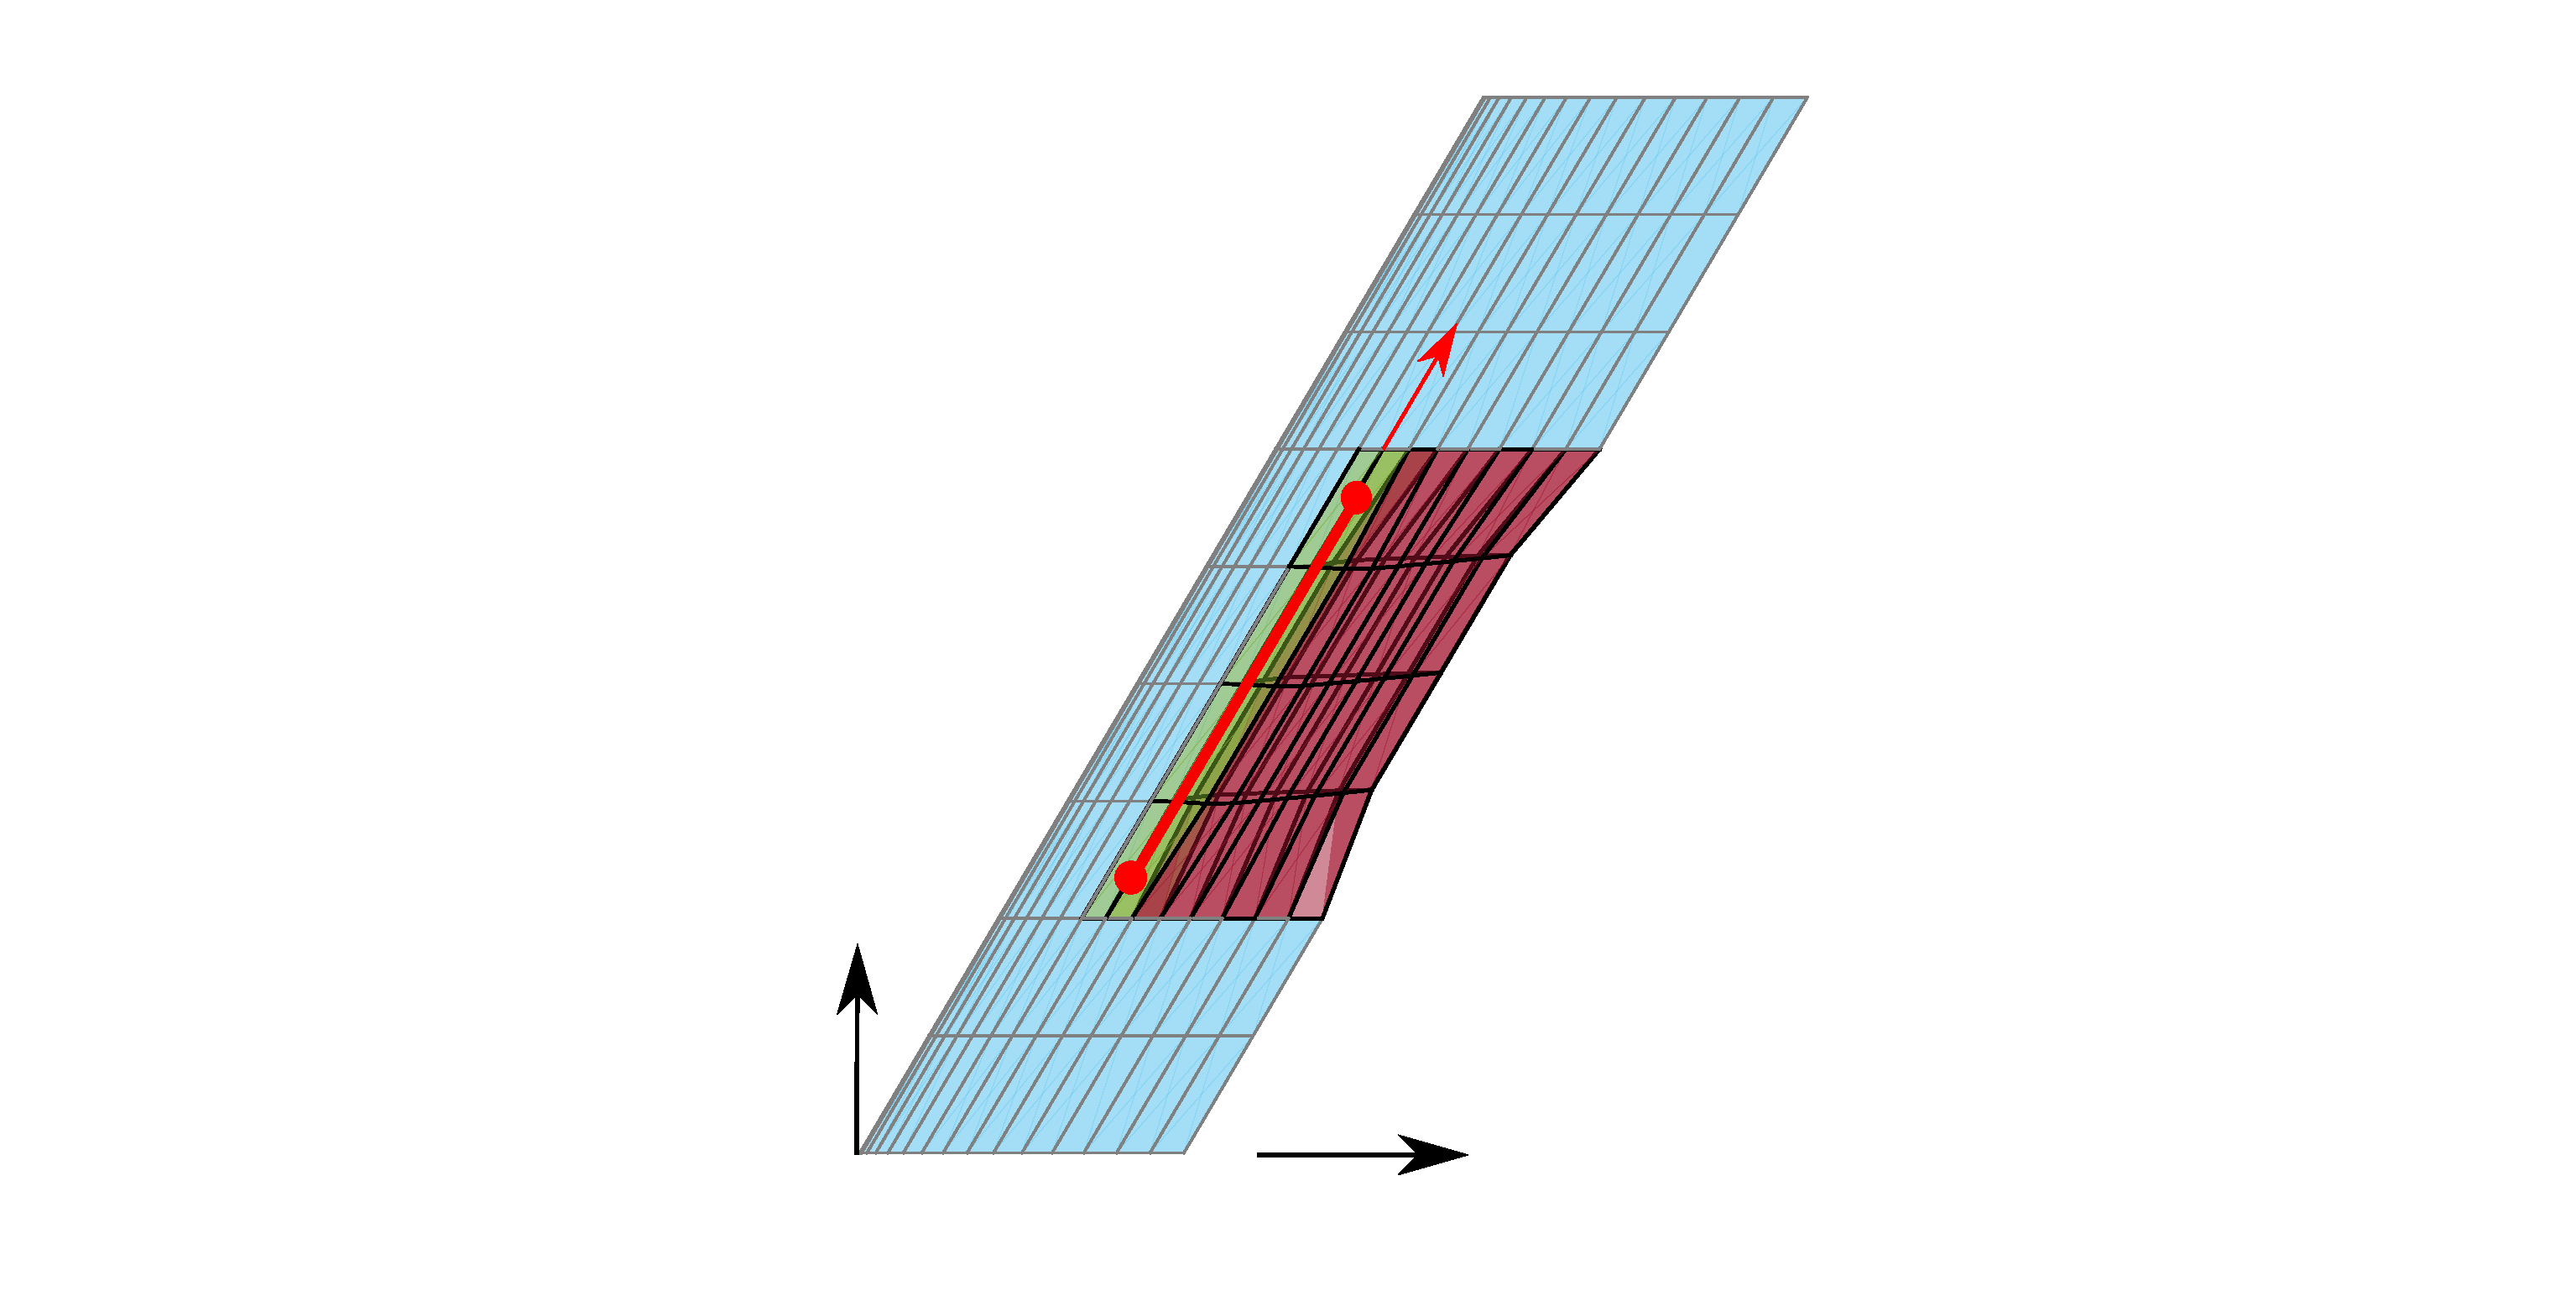
\includegraphics[width=\unitlength,page=1]{./images/hinge_ref_system.pdf}}%
    \put(0.52884911,0.07256303){\color[rgb]{0,0,0}\makebox(0,0)[lt]{\lineheight{1.25}\smash{\begin{tabular}[t]{l}$x_{dust}$\end{tabular}}}}%
    \put(0.27727265,0.12854856){\color[rgb]{0,0,0}\makebox(0,0)[lt]{\lineheight{1.25}\smash{\begin{tabular}[t]{l}$y_{dust}$\end{tabular}}}}%
    \put(0.5592075,0.33231148){\color[rgb]{0,0,0}\makebox(0,0)[lt]{\lineheight{1.25}\smash{\begin{tabular}[t]{l}$\Vec{h}$\end{tabular}}}}%
    \put(0.40960207,0.17181009){\color[rgb]{0,0,0}\makebox(0,0)[lt]{\lineheight{1.25}\smash{\begin{tabular}[t]{l}A\end{tabular}}}}%
    \put(0.50467099,0.31395518){\color[rgb]{0,0,0}\makebox(0,0)[lt]{\lineheight{1.25}\smash{\begin{tabular}[t]{l}B\end{tabular}}}}%
  \end{picture}%
\endgroup%

    \caption{hinge reference system for a swept wing}
     \label{fig:hingeref}
\end{figure}

The aerodynamic sections that are involved in the control surface are then the ones that satisfy the condition $y(A) < y(P) < y(B)$, where $y(P)$ is the ordinate of the $P_i-th$ aerodynamic mesh point expressed in the wind reference system. 
As in the 2D case, we can then define the three regions for each stripe identified at the previous point. The y coordinate of the origin of the sectional reference frame is determined by linear interpolation between points A and B. 
Points A and B corresponds to the user input \param{node_1} and \param{node_2}, respectively. The rotation axis is defined by $\Vec{h} = (B - A)$.

% input file
\begin{inputfile}[frame=single, caption={Parametric geometry for flapped wing}, label={file:parametric_example_flapped_wing.in}]
mesh_file_type = parametric
el_type = p
ScaleFactor = 1.0
offset = (/0.0 , 0.0,  0.0/)

mesh_symmetry = T
symmetry_point   = (/0.0 , 0.0,  0.0/)
symmetry_normal = (/0.0 , 1.0,  0.0/)

nelem_chord = 15
type_chord = cosineLE   ! uniform  cosineLE  cosineTE
starting_point = (/0.0,0.0,0.0/)
reference_chord_fraction = 0.25

n_hinges = 2
hinge = {
  Hinge_Tag = Aileron_right
  hinge_nodes_input = parametric      ! or from_file
  node_1 = (/ 1.4178, 1.4557, 0.3473/)  ! In the local ref.frame
  node_2 = (/ 2.4026  , 3.1615  , 0.6946/)
  n_nodes = 2
  ! }
  ! Hinge_Nodes_Input_From_File = {
  !   Node_File = hinge_node.dat
  ! }
  hinge_ref_dir = (/ 1.0, 0.0 , 0.0 /)
  hinge_offset  = 0.1
  hinge_spanwise_blending = 0.01
  hinge_rotation_input = function:sin
  hinge_rotation_function = {
    amplitude = 30.0    ! deg
    omega     =  12.5   ! rad/sec
    phase     =  0.0    ! deg
  }

hinge = {
  Hinge_Tag = Aileron_left
  hinge_nodes_input = parametric      
  node_2 = (/ 1.4178, -1.4557, 0.3473/)  
  node_1 = (/ 2.4026  , -3.1615  , 0.6946/)
  n_nodes = 2
  ! }
  ! Hinge_Nodes_Input_From_File = {
  !   Node_File = hinge_node.dat
  ! }
  hinge_ref_dir = (/ 1.0, 0.0 , 0.0 /)
  hinge_offset  = 0.1
  hinge_merge_tol = 0.01
  hinge_spanwise_blending = 0.01
  hinge_rotation_input = function:sin
  hinge_rotation_function = {
    amplitude = -30.0    ! deg
    omega     =  12.5    ! rad/sec
    phase     =  0.0     ! deg
  }


! First section
chord = 2
twist = 0.0
airfoil = NACA0012

! First region
span = 5.0
sweep = 30.0
dihed = 10.0
nelem_span = 20
type_span = uniform

! Second section
chord = 2
twist = 0.0
airfoil = NACA0012
\end{inputfile}

All the detailed parameters of the Hinged surfaces input file are: 
\begin{itemize}
    \item \param{n\_hinge}: \textit{required:} no.  \textit{multiple:} no. \textit{default:} 0.
    \textit{type:} integer
    
    Number of hinges and rotating parts (e. g. aileron) of the component.
    
    \item \param{hinge\_Tag}: \textit{required:} no. \textit{multiple:} same number as \param{n\_hinge} \textit{type:} string 
    
    name of the control surface.
    
    \item \param{hinge\_Nodes\_Input}: \textit{required:} yes. \textit{multiple:} no. \textit{type:} string
    
    type of hinge nodes input: \opt{parametric} or \opt{from\_file}. (TODO add details)
    
    \item \param{node_1} \textit{required:} yes. \textit{multiple:} no. \textit{type:} real array, length 3.
    
    First node of the hinge. Components in the local reference frame of the component.
    
    \item \param{node_2} \textit{required:} yes. \textit{multiple:} no. \textit{type:} real array, length 3.
    
    Second node of the hinge. Components in the local reference frame of the component.
    
    \item \param{hinge\_Ref\_Dir} \textit{required:} yes. \textit{multiple:} no. \textit{type:} real array, length 3. 
    
    Reference direction of the hinges, indicating zero-deflection direction in the local reference frame of the component.
    
    \item \param{hinge\_Merge\_Tol} \textit{required:} no. \textit{multiple:} no. \textit{type:} real. \textit{default:} 0.01
    
    Tolerance for adaptive hinge mesh in chord adimensional length. 
    
    \item \param{hinge\_Offset} \textit{required:} no. \textit{multiple:} no. \textit{type:} real. \textit{default:} 0.
    
    offset in the \param{hinge\_Ref\_Dir} needed for avoiding irregular behavior of the surface for large deflections.

    \item \param{hinge\_Spanwise\_Blending} \textit{required:} no. \textit{multiple:} no. \textit{type:} real. \textit{default:} 0.
    
    Blending in the spanwise direction needed for avoiding irregular behavior of the surface for large deflections.
    
    \item \param{hinge\_Rotation\_Input}
    \textit{required:} yes. \textit{type:} string.
    
    input type of the rotation: \opt{function}, \opt{from\_file} or \opt{coupling}. If the chosen option is \opt{coupling}, then the component must be coupled with preCICE (\param{Coupling} \opt{T}).
    
    \item \param{hinge\_Rotation\_Function}: \textit{required:} no. \textit{type:} string. 
    
    Parser for hinge input with simple functions; the supported functions are: \opt{function:const}, \opt{function:sin}, \opt{function:cos}. 
    \begin{itemize}
        \item \param{amplitude} \textit{required:} yes. \textit{type:} real. 
        
        amplitude of the rotation in degrees for constant, cosine and sine functions. 
        
        \item \param{omega} \textit{required:} yes. \textit{type:} real. \textit{default:} 0.0 
        
        Angular velocity of the rotation function in \si{\deg\per\second}, for constant?, cosine and sine functions.
        
        \item \param{phase} \textit{required:} yes. \textit{type:} real. \textit{default:} 0.0
        
        phase angle of the rotation function in \si{\deg}, for constant?, cosine and sine functions.
    \end{itemize}
    \item \param{hinge\_Rotation\_File} \textit{required:} no. \textit{type:} string. 
    
    Parser for hinge input from file
    
    \begin{itemize}
        \item \param{file_name} \textit{required:} yes. \textit{type:} string. 
        
        name of the file containing the input of the hinge rotation
    \end{itemize}
    
    \item \param{hinge\_Rotation\_Coupling} \textit{required:} no. \textit{type:} string.
    
    Parser for hinge input from coupling (see~\ref{subsec:DUSTpreCICE})
    
    \begin{itemize}
        \item \param{Coupling\_Node\_Subset} \textit{required:} no. \textit{type:} string.
        
        Define a subset of structural nodes to evaluate coupling: \opt{range} or \opt{from\_file}
        
        \item \param{Coupling\_Node\_First} \textit{required:} no. \textit{type:} integer. 
        
        If node subset is defined through \opt{range} input: first ID of the nodes
        
        \item \param{Coupling\_Node\_Last} \textit{required:} no. \textit{type:} integer. 
        
        If node subset is defined through \opt{range} input: last ID of the nodes
        
        \item \param{Coupling\_Node\_Filename} \textit{required:} no. \textit{type:} string.
        
        file collecting the IDs of the coupling nodes for hinge coupling
    \end{itemize}
    
    

    
\end{itemize}




\section{Pointwise mesh generation}
\label{sec:Pointwise_mesh_generation}
%
The \param{pointwise} mesh definition extends the capabilities of the \param{parametric} input. First, the reference line of the component is defined as a list of points connected with straight lines or Hermitian splines. The sections of a component are defined at each input points by means of their plane coordinates, their dimensions and rotation around an axis perpendicular to their own plane.
%
The input file is mainly composed of three sections: a generic section for the types of the aerodynamic elements and the symmetry and mirroring options, a section for the \param{point} list and a section for the \param{Line}. The parameters of the first section are very similar to the ones used in the \param{parametric} description, except for the \param{starting\_point}, that is not needed here, since the point with \param{Id}$=1$ is meant to be the first point of the reference line.
\newline \noindent
%
An example of input file for \param{pointwise}-defined component is provided in file \ref{file:pointwise_example_file.in}. The description of this file and all the parameters follows.
%

\begin{inputfile}[frame=single, caption={''Pointwise'' geometry definition }, label={file:pointwise_example_file.in}]
mesh_file_type = pointwise
el_type = p

mesh_symmetry = T
symmetry_point = (/0.0,0.0,0.0/)
symmetry_normal = (/0.0,1.0,0.0/)

mesh_mirror = F
mirror_point = (/0.0,0.0,0.0/)
mirror_normal = (/0.0,1.0,0.0/)

reference_chord_fraction = 0.0

mesh_flat = F

nelem_chord = 20
type_chord = cosineLE

! === Points ===
point = {
  Id = 1
  Coordinates = (/ 0.0 , 0.0 , 0.0 /)
  airfoil = NACA2412
  chord = 1.0
  twist = 5.0
  SectionNormal = yAxis
}
point = {
  Id = 2
  Coordinates = (/ 1.5 , 3.0 , 0.3 /)
  airfoil = NACA2412
  chord = 0.4
  twist = 0.0
  SectionNormal = yAxis
}
point = {
  Id = 3
  Coordinates = (/ 1.8 , 3.5 , 0.7 /)
  airfoil = NACA2412
  chord = 0.3
  twist = 0.0
  SectionNormal = referenceLine ! (default)
}
point = {
  Id = 4
  Coordinates = (/ 2.1 , 3.5 , 1.1 /)
  airfoil = NACA2412
  chord = 0.3
  twist = 0.0
  SectionNormal = referenceLine ! (default)
}
point = {
  Id = 5
  Coordinates = (/ 2.4 , 3.0 , 1.4 /)
  airfoil = NACA2412
  chord = 0.4
  twist = 0.0
  SectionNormal = yAxisNeg
  FlipSection = T
}
point = {
  Id = 6
  Coordinates = (/ 3.5 , 0.0 , 1.5 /)
  airfoil = NACA2412
  chord = 1.0
  twist = 5.0
  SectionNormal = yAxisNeg
  FlipSection = T
}

! === Lines ===
Line = {
  type = Straight
  EndPoints = (/ 1 , 2 /)
  Nelems = 5
}
Line = {
  type = Spline
  EndPoints = (/ 2 , 5 /)
  Nelems = 10
  ! see documentation for optional inputs
}
Line = {
  type = Straight
  EndPoints = (/ 5 , 6 /)
  Nelems = 5
}

\end{inputfile}
%
\begin{figure}[h!]
\centering
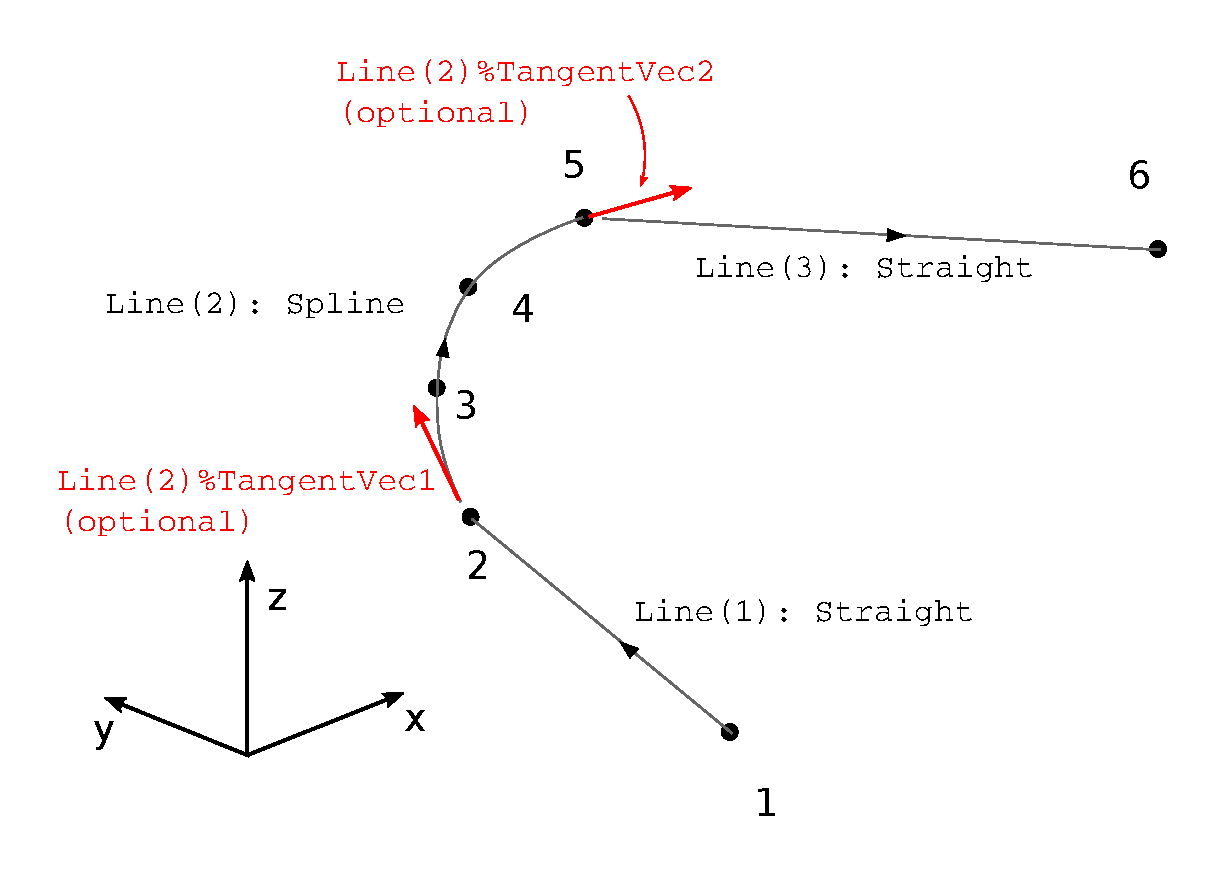
\includegraphics[width=.50\textwidth]{pointwise_2_referenceLine}
    \caption{Pointwise definition of a component: reference line by \param{point}s and \param{Line}s connecting them.}
\label{fig:pointwise_reference_line}
\end{figure}
%
\begin{figure}[h!]
\centering
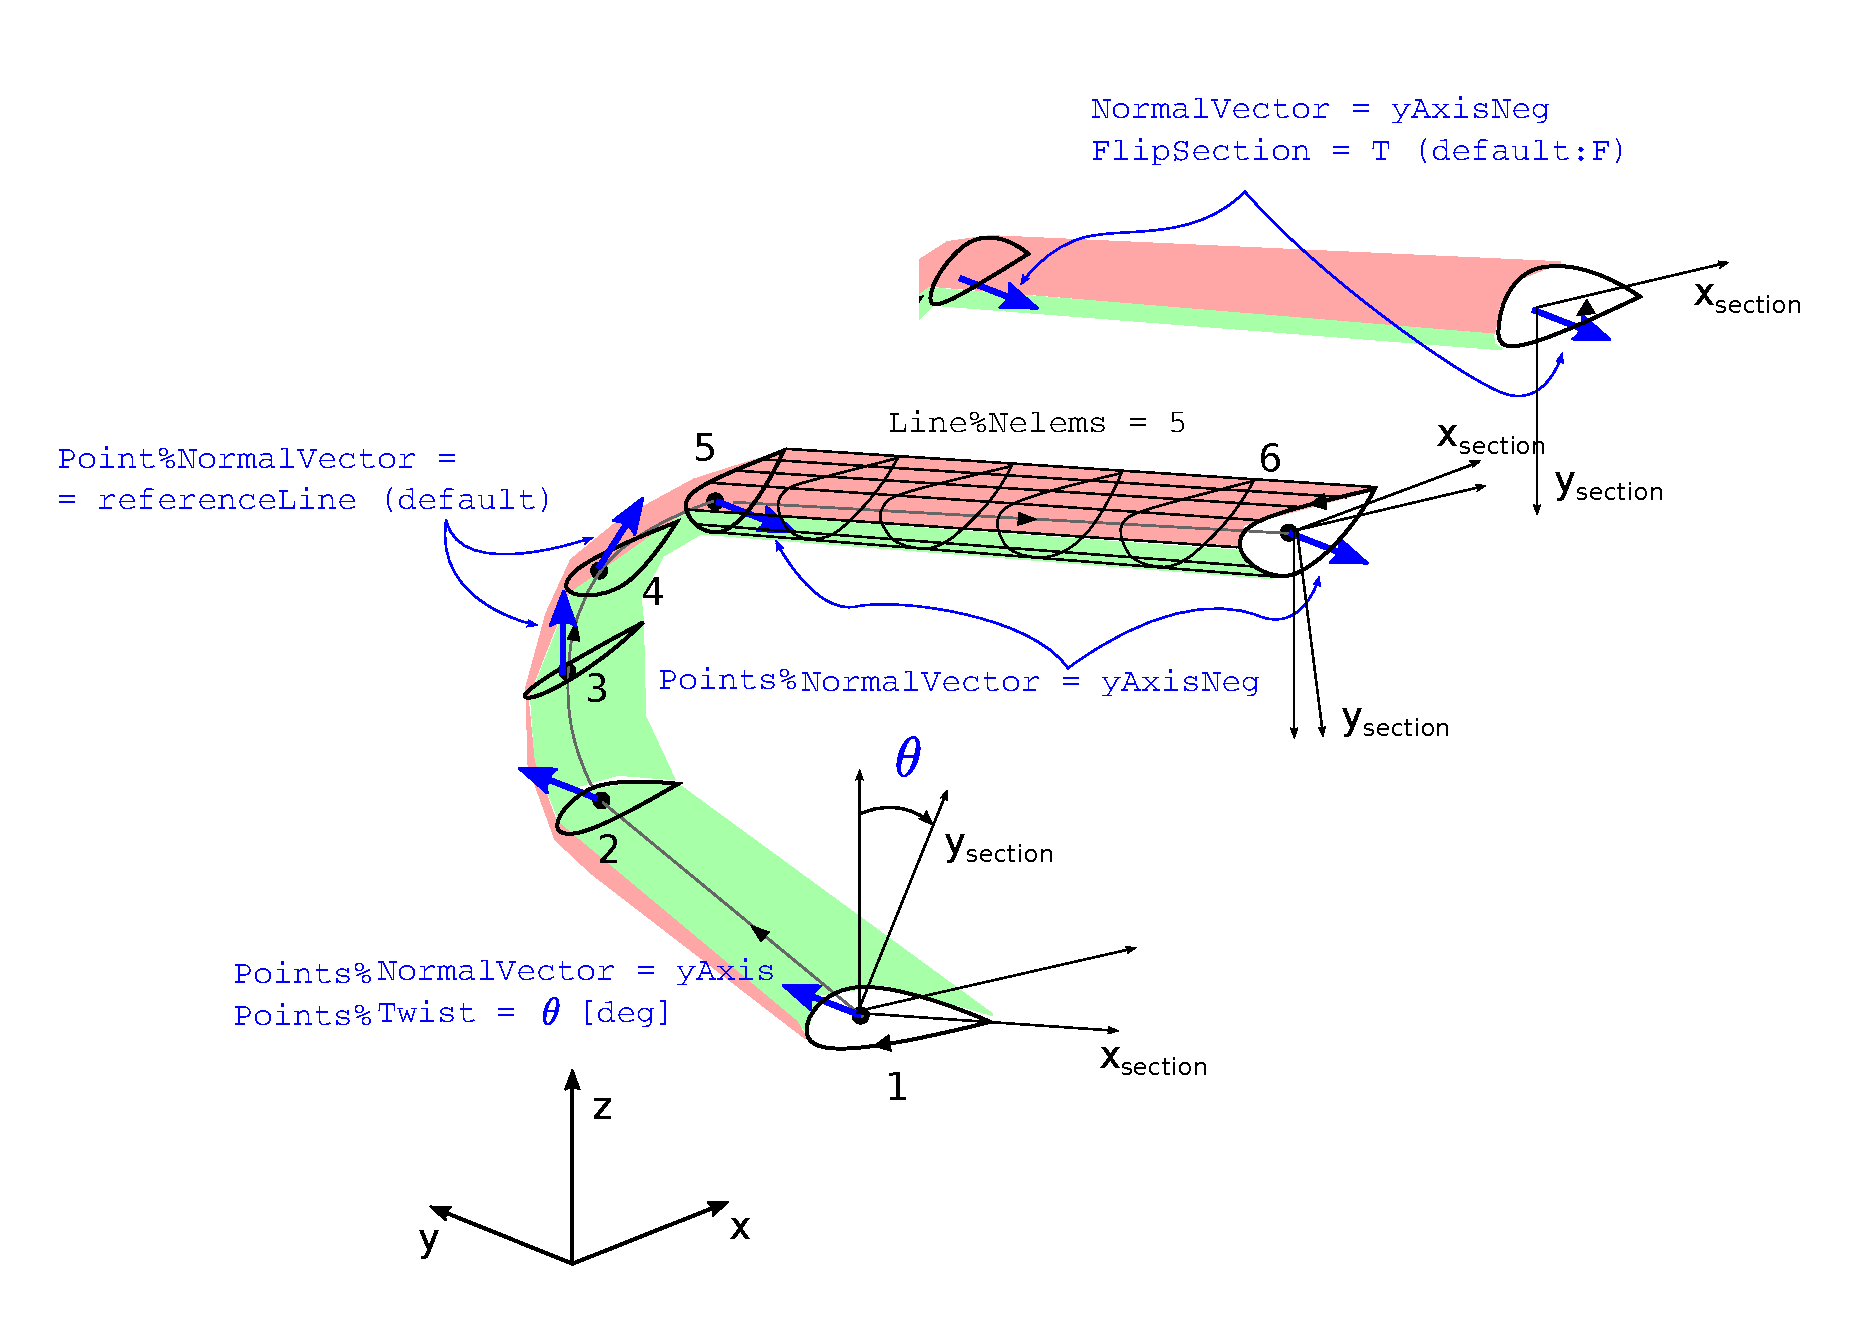
\includegraphics[width=.70\textwidth]{pointwise_3_component_flip}
    \caption{Pointwise definition of a component: section parameters (\param{airfoil}, \param{chord}, \param{twist}, \param{SectionNormal}) at \param{point}s of the reference line and the number \param{Nelems} of elements along the reference line for each \param{Line}. The parameter \param{FlipSection} can be set to \param{.true.} in order to flip the $y$-coordinate of the airfoil, in the section reference frame: the comparison between the goemetry with \param{FlipSection} equal to \param{F} or \param{T}  at \param{point} with \param{Id} = 5, 6 is shown in the picture for a non-symmetrical airfoil.}
\label{fig:pointwise_component}
\end{figure}


\begin{itemize}

\item \param{mesh_file_type}: \textit{required:} yes. \textit{multiple:} no. \textit{type:} string. 

Use \param{pointwise} for pointwise geometry.

\item \param{el_type}: \textit{required:} yes. \textit{multiple:} no. \textit{type:} character.

    type of the elements of the mesh. \opt{p} stands for surface panels to model solid bodies, \opt{v} stands for vortex lattice elements used to model flat surfaces, {\color{red}\opt{l} stands for lifting lines used to produce a 1D model of a lifting surface}. 

\item \param{mesh\_symmetry} \textit{required:} no. \textit{multiple:} no. \textit{default:} false. \textit{type:} logical.

Choose to reflect the mesh around a point and a direction. Useful to produce full meshes out of symmetrical half models. Keeps both the original and the symmetrical part. 

\item \param{symmetry\_point}: \textit{required:} only if \param{mesh\_reflection} is true. \textit{multiple:} no. \textit{default:} (0.0, 0.0, 0.0). \textit{type:} real array, length 3.

point around which to reflect the mesh.

\item \param{symmetry\_normal}: \textit{required:} only if \param{mesh\_reflection} is true. \textit{multiple:} no. \textit{default:} (0.0, 1.0, 0.0). \textit{type:} real array, length 3.

Direction in which to reflect the mesh.

\item \param{mesh\_mirror} \textit{required:} no. \textit{multiple:} no. \textit{default:} false. \textit{type:} logical.

Choose to mirror the mesh around a point and a direction. Same as \param{mesh\_symmetry} but does not keep both the original, i.e. the mesh is not doubled.

\item \param{mirror\_point}: \textit{required:} only if \param{mesh\_reflection} is true. \textit{multiple:} no. \textit{default:} (0.0, 0.0, 0.0). \textit{type:} real array, length 3.

point around which to mirror the mesh.

\item \param{mirror\_normal}: \textit{required:} only if \param{mesh\_reflection} is true. \textit{multiple:} no. \textit{default:} (0.0, 1.0, 0.0). \textit{type:} real array, length 3.

Direction in which to mirror the mesh.

\item \param{reference\_chod\_fraction} \textit{required:} no. \textit{multiple:} no. \textit{default:} 0.0 \textit{type:} real

Fraction of the chord at which to place the axis which will be rotated of the sweep and dihedral angles, and around which airfoils are twisted. 

\item \param{mesh\_flat} \textit{required:} no. \textit{multiple:} no. \textit{default:} true \textit{type:} logical

Used only in case of lifting lines (\opt{l}) elements. If enabled instead of generating lifting lies actually twisted according to the input twist, but rather a flat surface with only the normal vectors twisted according to the input twist. 

\item \param{nelem\_chord} \textit{required:} yes, if parametric. \textit{multiple:} no. \textit{type:} integer.

Number of elements in chord direction. Note: if the elements are vortex lattice $nelem\_chord$ elements will be generated, while in case of surface panels $2nelem\_chord$ elements will be produced, $nelem\_chord$ on the lower and $nelem\_chord$ on the upper side. In case of lifting lines this parameter is ignored.

\item \param{type\_chord} \textit{required:} no. \textit{multiple:} no. \textit{default:} \param{uniform} \textit{type:} string.

type of subdivision in the chord-wise direction. Can be \opt{uniform} for a uniform distribution, \opt{cosine} for a cosine distribution, refined both on the leading and trailing edge, \opt{cosineLE} for a half cosine refined only on leading edge or \opt{cosineTE} for a half cosine refined only on the trailing edge. 

\end{itemize}
%
A list of \param{point} groups follows. These points are used to describe the reference line of the component. The parameters of a \param{point} element are:
\begin{itemize}

\item \param{Id} \textit{required}: yes, \textit{multiple}: no, \textit{type}: integer.

    Id. number of the \param{point}, used in the point-to-line connectivity defined in \param{Line} groups.

\item \param{Coordinates}  \textit{required}: yes, \textit{multiple}: no, \textit{type:} real array, length 3.

    Coordinates of the point in the local reference frame of the component.
    
\item \param{airfoil}  \textit{required}: yes, \textit{multiple}: no, \textit{type}: string.

    Same as in the parametric definition of a component. To be used for vortex lattices or surface panels
    
\item \param{airfoil\_table}  \textit{required}: yes, \textit{multiple}: no, \textit{type}: string.

    Same as in the parametric definition of a component. To be used for lifting lines only in place of \param{airfoil}

\item \param{chord}  \textit{required}: yes, \textit{multiple}: no, \textit{type}: real.

    Define section dimensions, by its chord length.

\item \param{twist}  \textit{required}: yes, \textit{multiple}: no, \textit{type}: real.

    Angle of twist, in degrees, of the airfoil section. rotation around the vector that is normal to the plane of the section.

\item \param{SectionNormal} \textit{required}: no, \textit{multiple}: no , \textit{default}: \param{referenceLine} , \textit{type}: string.

    String to define the plane of the section. It can be: \param{referenceLine}, for sections perpendicular to the reference line; \param{yAxis}, \param{yAxisNeg} for sections perpendicular to the $y$-axis or $-y$-axis of the component local reference frame; \param{vector}, to define a generic vector. 

\item \param{SectionNormalVector} \textit{required}: only if \param{SectionNormal = vector}, \textit{multiple}: no, \textit{type}: real array, length 3.

    Components of the normal vector of the section, if \param{SectionNormal = vector}.

\item \param{FlipSection} \textit{required}: no, \textit{multiple}: no, \textit{default}: \param{F} , \textit{type}: logical.

   Flip the $y$ coordinates in the section reference frame. Meant to help the pointwise definition of close wing configurations.

\end{itemize}
%
A list of \param{Line} groups follows. These lines are used to build the reference line of the component connecting the points defined above. The parameters of a \param{Line} element are:
\begin{itemize}

\item \param{type} \textit{required}: yes, \textit{multiple}: no, \textit{type}: string.

    Line type. It can be: \param{Straight} for straight lines, \param{Spline} for Hermitian splines.

\item \param{EndPoints}  \textit{required}: yes, \textit{multiple}: no, \textit{type}: integer array, lenght 2.

    \param{Id} numbers of the beginning and ending \param{point}s of the line. For \param{Straight} lines, this two numbers must be consecutive. For \param{Spline}s the spline is built using these ones as the first and last points and all the points with \param{Id} in between as interior points, so that they must exist in the point list.

\item \param{Nelems}  \textit{required}: yes, \textit{multiple}: no, \textit{type}: integer.

    Number of elements in the direction of the reference line belonging to this region.

\item \param{type\_span} \textit{required}: no, \textit{multiple}: no, \textit{default}: \param{uniform}, \textit{type}: string.

    type of refinement of the elements in the spanwise direction. As for the chordwise direction, the options are \opt{uniform} for a uniform distribution, \opt{cosine} for a cosine refinement both inboard and outboard, and \opt{cosineIB} and \opt{cosineOB} for half cosine refinement only inboard or outboard. 
  
\item \param{TangentVec1} \textit{required}: if \param{Line\%type = Spline} and \param{Line\%EndPoints(1) = 1}, \textit{multiple}: no, \textit{type}: real array, length 3. 

    Tangent vector at the first point of a \param{Spline}. This is an optional input for \param{Spline}. If this field is not present, the spline inherits the tangent vector from the neighboring line (that must be a \param{Straight} line).

\item \param{TangentVec2} \textit{required}: if \param{Line\%type = Spline} and \param{Line\%EndPoints(2)} is the last point of the reference line, \textit{multiple}: no, \textit{type}: real array, length 3. 

    Tangent vector at the last point of a \param{Spline}. This is an optional input for \param{Spline}. If this field is not present, the spline inherits the tangent vector from the neighboring line (that must be a \param{Straight} line).

\item \param{Tension} \textit{required}: no, \textit{multiple}: no, \textit{default}: 0.0 , \textit{type}: real.

    \param{Tension} parameter of the Hermitian \param{Spline}.

\item \param{Bias} \textit{required}: no, \textit{multiple}: no, \textit{default}: 0.0 , \textit{type}: real.

    \param{Bias} parameter of the Hermitian \param{Spline}.

\end{itemize}

\subsection{Hermitian splines}
The Hermitian splines by the following expression,
\begin{equation}
\mathbf{r}_i(t) = \mathbf{r}_{i-1} h_0(t) + \mathbf{r}_{i} h_1(t) +
                  \mathbf{d}_{i-1} h_2(t) + \mathbf{d}_{i} h_3(t) \ ,
\end{equation}
where $h_i(t), \ i=0:3$ are the Hermitian functions, the points $\mathbf{r}_i$ are the points to be interpolated, $\mathbf{d}_i$ the approximation of the derivatives at the interpolation points. For the interior points of a spline,
\begin{equation}
\begin{aligned}
\mathbf{d}_i & = 0.5 ( \mathbf{r}_{i+1} - \mathbf{r}_{i  } ) \ (1-\param{Bias}) (1-\param{Tension}) \\
             & + 0.5 ( \mathbf{r}_{i  } - \mathbf{r}_{i-1} ) \ (1+\param{Bias}) (1-\param{Tension}) \ .
\end{aligned}
\end{equation}
The \param{Bias} parameter is a weight on the finite difference computed using forward and backward differences, while \param{Tension} acts like a tensile action on the spline, see figure \ref{fig:spline_tension}.
\begin{figure}[h!]
\centering
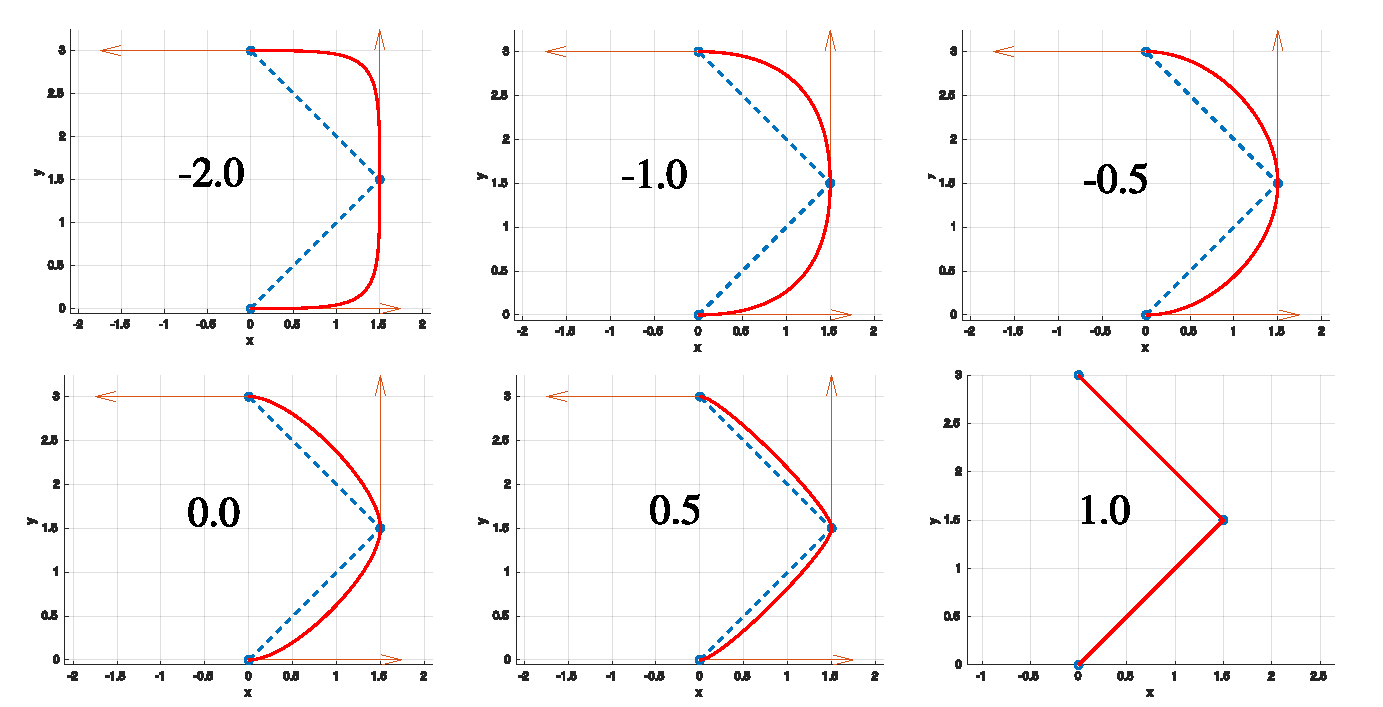
\includegraphics[width=.80\textwidth]{spline_tension}
    \caption{Influence of the \param{Tension} parameter on the shape of the spline interpolating points $(0,0)$, $(1.5,1.5)$ $(0,3)$, with prescribed horizontal derivatives at the end points.}
\label{fig:spline_tension}
\end{figure}

\subsection{Limitations and errors in the pointwise definition of a component}
So far, the code has the following limitations:
\begin{itemize}
    \item if \param{mesh\_symmetry = T}, the last section of the component can be joined only if the first section is joined. A workaround is to flip the order of the points and reverse the direction of the reference line, in order to have the first section corresponding to the previously defined last section and viceversa, so that the desired sections are joined. No limitation exists if both the first and last sections belong to the symmetry plane and are joined.
    
    \item it is not possible to join two consecutive \param{Spline}s lines. So far, \param{Spline}s are meant to join \param{Straight} lines or to be the first or last line. However a single spline can be used to join an arbitrary number of points. 
    
    \item it is not possible to define the first or last line as a \param{Spline}, without providing the tangent vector at the free end, i.e. the \param{TangentVec1} must be provided to the first line, \param{TangentVec2} to the last line. Spline routines have the capability to treat free ends, with second derivative equal to zero, but some modifications in the pointwise definition of a component are still needed to allow for free ends.
    
\end{itemize}

\subsection{Bodies of Revolution}
\label{subs:Bodies_Revolution}
A simple parametric mesh generation to create bodies of revolution is available. With this type of input is possible to generate bodies by revolving an user provided profile or cylindrical bodies with smooth tapered ends only with parametric inputs. An example of input file for this kind of parametric input is available in file 

\begin{inputfile}[frame=single, caption={Boies of revolution geometry definition }, label={file:revolution_example_file.in}]
mesh_file_type = revolution
el_type = p

mesh_symmetry = T
symmetry_point = (/0.0,0.0,0.0/)
symmetry_normal = (/0.0,1.0,0.0/)

mesh_mirror = F
mirror_point = (/0.0,0.0,0.0/)
mirror_normal = (/0.0,1.0,0.0/)

!mesh_file = rev_profile.dat

rev_length = 5.0
rev_nose_radius = 1.0
rev_radius = 0.7
rev_nelem_long = 30
rev_nelem_rev = 10

\end{inputfile}

\begin{itemize}

\item \param{mesh_file_type}: \textit{required:} yes. \textit{multiple:} no. \textit{type:} string. 

Use \param{revolution} for bodies of revolution

\item \param{el_type}: \textit{required:} yes. \textit{multiple:} no. \textit{type:} character.

    Only \opt{p} for surface panels is supported for bodies of revolution.

\item \param{mesh\_symmetry} \textit{required:} no. \textit{multiple:} no. \textit{default:} false. \textit{type:} logical.

Choose to reflect the mesh around a point and a direction. Useful to produce full meshes out of symmetrical half models. Keeps both the original and the symmetrical part. 

\item \param{symmetry\_point}: \textit{required:} only if \param{mesh\_reflection} is true. \textit{multiple:} no. \textit{default:} (0.0, 0.0, 0.0). \textit{type:} real array, length 3.

point around which to reflect the mesh.

\item \param{symmetry\_normal}: \textit{required:} only if \param{mesh\_reflection} is true. \textit{multiple:} no. \textit{default:} (0.0, 1.0, 0.0). \textit{type:} real array, length 3.

Direction in which to reflect the mesh.

\item \param{mesh\_mirror} \textit{required:} no. \textit{multiple:} no. \textit{default:} false. \textit{type:} logical.

Choose to mirror the mesh around a point and a direction. Same as \param{mesh\_symmetry} but does not keep both the original, i.e. the mesh is not doubled.

\item \param{mirror\_point}: \textit{required:} only if \param{mesh\_reflection} is true. \textit{multiple:} no. \textit{default:} (0.0, 0.0, 0.0). \textit{type:} real array, length 3.

point around which to mirror the mesh.

\item \param{mirror\_normal}: \textit{required:} only if \param{mesh\_reflection} is true. \textit{multiple:} no. \textit{default:} (0.0, 1.0, 0.0). \textit{type:} real array, length 3.

Direction in which to mirror the mesh.

\item \param{mesh_file}: \textit{required:} no. \textit{multiple:} no. \textit{type:} string.

name of an ascii file containing the point list describing the curve or profile to revolve, which will be revolved around the local x axis. If the input is present, the rest of the inputs are neglected and the body is built revolving the provided profile, otherwise if  \param{mesh_file} is not present, the parametric input is employed

\item \param{Rev\_Length}: \textit{required:} yes if \param{mesh_file} is not present. \textit{multiple:} no. \textit{type:} real.

Length of the parametric body of revolution, from tip to tip.

\item \param{Rev\_Nose\_Radius}: \textit{required:} yes if \param{mesh_file} is not present. \textit{multiple:} no. \textit{type:} real.

radius of the smooth circular tapering at the ends of the cylindrical body of revolution

\item \param{Rev\_Radius}: \textit{required:} yes if \param{mesh_file} is not present. \textit{multiple:} no. \textit{type:} real.

radius of the central cylindrical section of the body of revolution

\item \param{Rev\_Nelem\_Long}: \textit{required:} yes if \param{mesh_file} is not present. \textit{multiple:} no. \textit{type:} integer.

Number of elements in the longitudinal direction of the body of revolution


\item \param{Rev\_Nelem\_Rev}: \textit{required:} yes. \textit{multiple:} no. \textit{type:} integer.

Number of elements in the revolution direction. 


\end{itemize}


\section{Trailing Edge}
\label{sec:TrailingEdge}

The trailing edge is the line from which the wake is shed from the geometry elements. It is meant to represent the location where the thin vortical layer leaves a lifting body when the boundary layer is still attached. In the \DUST \ preprocessor the trailing edge is identified geometrically, possibly according to a set of parameters. 

In case of paranetrically generated elements, which represent extruded airfoils, the trailing edge is simply generated connecting all the trailing edge of the two (or mono) dimensional sections that compose the parametric geometry.

In case of unstructured surface meshes, the preprocessor proceeds by trying to geometrically identify the trailing edge in sharp corners between elements. 

Considering the (rather common) possibility that the trailing edges are left open, i.e. with element edges not geometrically connected and/or not logically connected in the connectivity, first the \DUST preprocessor merges the close nodes and generates an alternative connectivity taking into account the new connections. 
This merging is just functional to the definition of the trailing edge, and will be discarded after the trailing edge had been identified. To control the merging, the parameter \param{tol_se_wing} can be declared in the preprocessor input file, to be applied globally, or in each (or some) single geometry input file to be applied to a single component. Each pair of nodes separated by a distance lower than \param{tol_se_wing} will be merged in this phase.

After merging the mesh the new connectivity will be employed to identify the edges belonging to the trailing edge. The edges between two elements whose normal vectors are \emph{sufficiently} opposed are marked as trailing edge. In particular, the edge connecting the elements $i$ and $j$ is a trailing edge if 
\begin{equation}
    \Vec{n}_i\cdot\Vec{n}_j < \text{\param{inner_product_te}},
\end{equation}
where $\Vec{n}_i,\Vec{n}_j$ are the normal unit vectors of the respective elements.

Moreover during the preprocessing also the direction of the first wake panel is decided. During the simulation the whole wake is advected according to the velocity generated by the singularities of the bodies and the wake, however the first wake panel is geometrically pre-determined and its intensity is implicitly solved alongside the rest of the singularities of the body surfaces. The first panel starts from the trailing adge and its nodes, and its length is decided during the simulation, however the direction alongside it is stretched from the trailing edge is determined in the preprocessor. 

If no specific indication is given, the direction of the first implicit wake panel is the average of the two edges directions from the upper and lower elements connected at the trailing edge node. It is however possible to alter this behaviour  by setting \param{proj_te} to true. Then the user must provide a direction vector with \param{proj_te_vector}, which identifies the direction in which to project the first panel direction if \param{proj_te_dir} is \opt{parallel}, or is the normal to the plane in which to project the first panel direction if  \param{proj_te_dir} is \opt{normal}.




\section{Actuator Disks}
\label{sec:ActuatorDisks}
Actuator disks are built employing a parametric input file just as file \ref{file:parametric_geo_file.in} but with different parameters, shown in file \ref{file:actdisk_geo_file.in} 

\begin{inputfile}[frame=single, caption={actdisk\_geo\_file.in}, label={file:actdisk_geo_file.in}]
mesh_file_type = parametric
el_type = a

radius = 2.5
nstep = 20
Axis = 3
traction = 10.0
\end{inputfile}


All the detailed parameters of the geometry input file for parametric actuator disks are:
\begin{itemize}
\item \param{mesh_file_type}: \textit{required:} yes. \textit{multiple:} no. \textit{type:} string. 

Use \param{parametric} for parametric geometry.

\item \param{el_type}: \textit{required:} yes. \textit{multiple:} no. \textit{type:} character.

type of the elements of the mesh. For actuator disks must be \param{a}

\item \param{radius}: \textit{required:} yes. \textit{multiple:} no. \textit{type:} real.

radius of the actuator disk.

\item \param{nstep}: \textit{required:} yes. \textit{multiple:} no. \textit{type:} integer.

Number of straight segments used to discretize the circle of the actuator disk.

\item \param{Axis}: \textit{required:} yes. \textit{multiple:} no. \textit{type:} integer.

Which of the three axis of the reference frame to use as axis of the rotor. The reference frame is the one specified for the component in the preprocessor input, file \ref{file:dust_pre.in}

\item \param{traction}: \textit{required:} yes. \textit{multiple:} no. \textit{type:} real.

traction of the actuator disk.
\end{itemize}



